\documentclass{ieeeaccess}
\usepackage{cite}
\usepackage{amsmath,amssymb,amsfonts}
\usepackage{algorithmic}
\usepackage{graphicx}
\usepackage{textcomp}
\usepackage{multirow}
\usepackage{array}
\def\BibTeX{{\rm B\kern-.05em{\sc i\kern-.025em b}\kern-.08em
    T\kern-.1667em\lower.7ex\hbox{E}\kern-.125emX}}
\begin{document}
%\history{Date of publication xxxx 00, 0000, date of current version xxxx 00, 0000.}
%\doi{10.1109/ACCESS.2017.DOI}

\title{Enhancing the Performance of URLLC Uplink Transmissions}
\author{\uppercase{Trung-Kien Le}\authorrefmark{1},
\uppercase{Umer Salim\authorrefmark{2}, and Florian Kaltenberger}.\authorrefmark{1},
}
\address[1]{EURECOM, Sophia Anitpolis, France (e-mail: author@eurecom.fr)}
\address[2]{TCL Mobile, Sophia Antipolis, France (e-mail: author@tcl.com)}

\tfootnote{This work was supported in part by TCL and H2020 project 5GENESIS (5genesis.eu).}

\markboth
{Trung-Kien Le \headeretal: Enhancing the Performance of URLLC Uplink Transmissions}
{Trung-Kien Le \headeretal: Enhancing the Performance of URLLC Uplink Transmissions}

\corresp{Corresponding author: Trung-Kien Le (e-mail: Trung-Kien Le@eurecom.fr).}

\begin{abstract}
The unprecedented growth of technology leads to the appearance of new applications such as virtual reality, autonomous driving, real time remote surgery, to name but a few. These applications have stringent requirements of reliability and latency specified by The 3rd Generation Partnership (3GPP) in the category of Ultra-Reliable Low-Latency Communication (URLLC). Heavy changes in physical layer design of 5G Standardization were introduced to satisfy these requirements, yet many more still be required. In this article, the technical challenges in URLLC uplink (UL) transmission and the proposed techniques to overcome them are described. The first challenge is the multiplexing of enhanced mobile broad band (eMBB) and URLLC. The collision between these two services is solved by introducing a cancellation indication (CI) or an overlap indication with an explicit Hybrid automatic repeat request (HARQ) feedback structure or an additional scheduling request (SR). The second challenge is to ensure the configured number of repetitions in URLLC UL configured-grant (CG) transmission to ensure a certain reliability target. Three techniques are proposed to use reserved resources, an explicit HARQ feedback or an additional SR.
\end{abstract}

\begin{keywords}
5G, configured-grant resources, eMBB and URLLC multiplexing, repetitions, reserved resources, uplink scheduling scheme, URLLC
\end{keywords}

\titlepgskip=-15pt

\maketitle

\section{Introduction}
\label{I}
The development of technology in the recent industrial revolution has paved the way for the emergence of new applications such as virtual reality, autonomous vehicles, real time remote surgery, to name but a few. In parallel to this, there is an ever growing demand for large throughput, and the promise of internet of things (IoT) objects. To cover such wide variety of use cases with diverse requirements, 3GPP defined three service paradigms for 5G: eMBB, Massive Machine-Type Communication (mMTC) and URLLC. Among these three service categories, URLLC raises the most challenge because it has to deal with two conflicting factors at the same time: reliability and latency. For 3GPP Release-15, which becomes the fundamental release of 5G new-radio (NR), the URLLC requirements are specified in \cite{ref1}: ``A general URLLC reliability requirement for one transmission of a packet is 10\textsuperscript{-5} for 32 bytes with a user plane latency of 1 ms''. In the next release of 3GPP (Release 16), the more stringent requirements are targeted: ``Higher reliability (up to 10\textsuperscript{-6}), higher availability, short latency in the order of 0.5 to 1 ms, depending on the use cases (factory automation, transport industry and electrical power distribution)''\cite{ref2}.

In order to achieve URLLC requirements, some principal techniques are specified in 3GPP Release 15 finalized in December 2018.

The first aspect is related to the usage of flexible sub-carrier spacing (SCS). In LTE, the value of SCS is fixed at 15 kHz. In contrast, the value of SCS in 5G can be 15 kHz, 30 kHz, 60 kHz, 120 kHz and 240 kHz \cite{ref3}. This results in short symbol and slot. As data is normally scheduled at slot level, the network becomes very reactive to UL and downlink (DL) traffic demands. Thus, the time alignment and transmission of packets becomes much faster compared to that of LTE. 

The second aspect is related to mini-slot based transmissions. It has been agreed that a packet can be scheduled to be transmitted in DL or UL in the interval of one or several symbols instead of the whole slot as LTE \cite{ref4}.

The third aspect is the standardization of the UL configured grant (CG) transmissions. In the conventional grant-based (GB) transmission, when a user equipment (UE) has data to transmit, it must send scheduling request (SR) to the base station (gNB) then receives UL grant from the gNB for UL resource allocation. However, in a CG transmission, the UE is configured with the periodic transmission resources by the gNB so it can transmit data immediately in these resources without the presence of SR and UL grant \cite{ref5}.This transmission mode helps to reduce the processing and transmission time of SR and UL grant that brings significant latency advantage to UL transmission.

A fourth aspect is the flexible configurable HARQ timing. Contrary to LTE 4 m-sec fixed duration between data transmission and its associated HARQ response, 5G allows flexible configuration of HARQ timing, even permitting the same slot HARQ response for some low latency applications.

These new features have allowed achieving significantly large quality of service (QoS) requirements compared to what was possible with 4G. Yet, the URLLC applications described previously may still benefit with improved link performance. 3GPP Release-16, currently under standardization, is trying to make further progress on some important topics such as PDCCH reliability, PUSCH enhancements, eMBB and URLLC multiplexing, and UL CG enhancements etc. 

\subsection{Main contributions}

This work contributes to solve two major problems relevant to URLLC, acknowledged by 3GPP. Section \ref{II} deals with the first problem of URLLC performance's deterioration in eMBB and URLLC multiplexing. The straight forward approach for the operators is to reserve bandwidths (BWs) (or parts of BWs) for different service types. This will lead to large degradation in spectral efficiency, making it important to multiplex different service types.  The first scenario of multiplexing between GB eMBB and CG URLLC is considered in \ref{IIB}. In the literature, some techniques have been proposed such as increasing power level of URLLC transmission, updating dynamically URLLC transmission parameters, making URLLC transmission wait until the next available CG regions, using cancellation indication (CI) and using successive interference cancellation (SIC) receiver. Each technique has its own disadvantages that will be discussed in detail in Section \ref{IIBN}. Section \ref{IIB2} and \ref{IIB3} summarize two techniques that we proposed in \cite{ad99}. The first technique uses an overlap indication and an explicit feedback structure. The second technique uses an overlap indication and an additional SR. These techniques reduce packet loss due to interference and Demodulation Reference Signal (DMRS) miss-detection. Subsequently, in Section \ref{IIA}, the paper extends the work in \cite{ad99} by analyzing and developing the techniques to solve the problems in the second scenario of the multiplexing between GB eMBB and GB URLLC UEs.  A bit flag is included in UL grants to specify the UEs that need to monitor CI on mini-slot level. The selection between group common (GC) CI and UE-specific CI is explained in the subsection about CI design. These techniques reduces energy consumption at the UEs and resource consumption in the system.

Section \ref{III} copes with another important problem of URLLC related to CG transmissions. These UEs may be configured with CG transmissions frequently to avoid scheduling delays, and with multiple repetitions for the same transport block (TB) to ensure a certain reliability. As packet arrival at the UEs is not aligned to system timing, packets appearing in the middle of the interval will either have to wait for the next interval to transmit the configured number of repetitions or transmit fewer repetitions in the current interval. The former may be a problem for latency whereas the latter may lead to reliability issue. Some techniques have been proposed in the literature and 3GPP meetings such as using multiple configurations, allowing the repetitions to cross boundary of a HARQ process, and using shared resources for repetitions. The description and analysis of these techniques are written in Section \ref{IIIBN}. Subsequently, three different techniques to solve this problem or at least alleviate the harmful effect of a smaller number of repetitions transmitted that we proposed in \cite{b9} and \cite{ad100} are described and compared with each other. Some new developments and the way to combine these technique to use at the same time are also shown in this part. The first technique in Section \ref{IIIB} uses reserved resources so that the UE can use them to transmit the repetitions until it reaches the configured number. The sizes of the reserved resources are optimized based on their positions. The further development of this scheme with SIC receiver is presented in this paper. The second technique in Section \ref{IIIC} demands the UE to activate explicit HARQ feedback structure if it cannot do all repetitions as configured. This structure helps reduce the probability of packet loss due to DMRS miss-detection. The third technique in Section \ref{IIID} asks the UE to transmit an additional SR in case of a smaller number of repetitions transmitted. This SR provides another chance for the gNB to recognize UE appearance so that packet loss's probability decreases. 

\section{UL eMBB and URLLC multiplexing}\label{II}

In UL transmission, there are the cases that an UL transmission at the eMBB UE has been already dynamically scheduled by UL grant from the gNB. However, this transmission might collide with an URLLC transmission. In the first scenario, another URLLC UE is scheduled to transmit in the resources that were already allocated to the eMBB so that the URLLC transmission can attain the strict requirements. It causes a collision between the eMBB1 and the URLLC UE1 in Fig.~\ref{fig21}. In the second scenario, an URLLC UE transmits in the CG resources without the gNB's awareness and collides with the eMBB UE that is also scheduled to transmit in those resources as the collision between the eMBB UE2 and URLLC UE2 in Fig.~\ref{fig21}. The collisions in these two scenarios degrade the performance of both two kinds of transmission, especially for the URLLC transmission. The causes and solutions for these two scenarios are going to be explained in the next subsections.

\begin{figure}[htbp]
\centerline{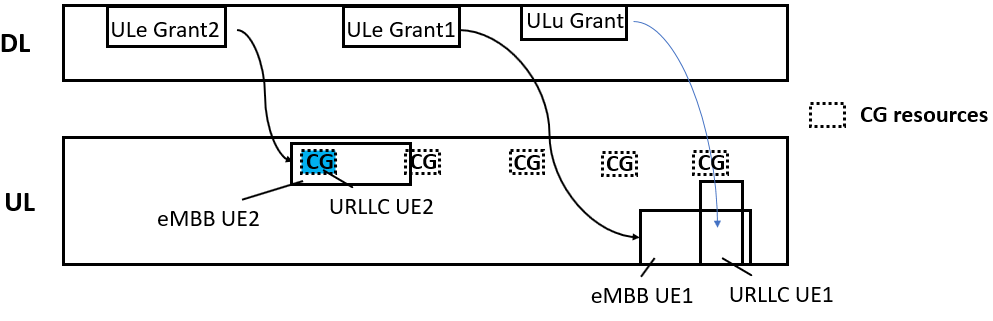
\includegraphics[scale=0.33]{fig21.PNG}}
\caption{Two scenarios of collisions between the eMBB UEs and URLLC UEs.}
\label{fig21}
\vspace{-5mm}
\end{figure}

\subsection{GB eMBB and CG URLLC multiplexing}\label{IIB}
\subsubsection{Problem formulation}\label{IIB1}
As mentioned in Section \ref{I}, CG resources is one option for URLLC transmission to reduce transmission and processing time of SR and UL grant. However, the gNB does not have information of the arrival of packets at the UE side. Therefore, there is the case that the UE does not use the CG resources because it has no arriving data to transmit and those resources would be wasted. It is harmful to the network if it has many active UEs (eMBB and URLLC UEs). In that scenario as in Fig.~\ref{fig1}, the gNB dynamically schedules some of the eMBB UEs to use the CG resources overlapping with other URLLC UEs.

\begin{figure}[htbp]
\centerline{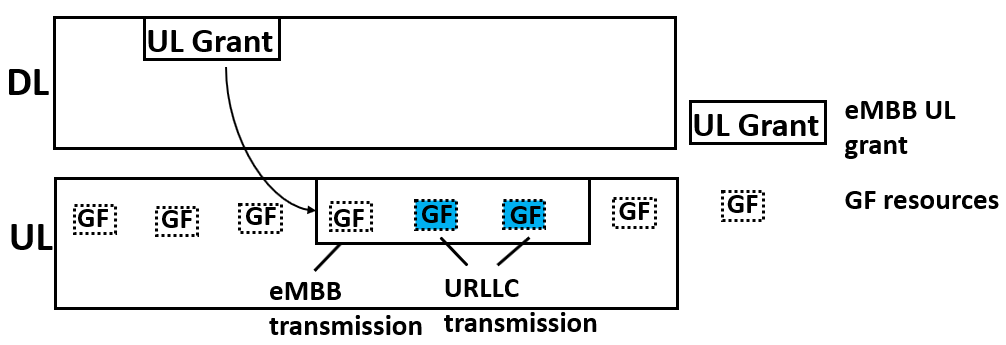
\includegraphics[scale=0.32]{fig1.PNG}}
\caption{A collision of UL URLLC CG transmission with eMBB transmission in case of Frequency Division Duplex (FDD).}
\label{fig1}
\end{figure}

Thanks to the multiplexing of the eMBB UEs into the CG resources, the system attains a higher resource utilization when the URLLC UEs have no data to transmit in those resources. Nevertheless, there might be a collision between eMBB and URLLC data in the CG regions if an URLLC UE needs to transmit an arriving packet immediately to meet latency requirement. A potential interference between eMBB and URLLC UEs that is unknown to the gNB at the scheduling moment deteriorates reliability of URLLC transmission. As a result, a decoding error at the gNB is more likely to happen. It may make the URLLC transmission be unable to achieve reliability target. The URLLC transmission in the CG resources is not prior known by the gNB. A CI as described in Section \ref{IIA} cannot be used to stop the eMBB UE at the time of URLLC transmission.

The situation in eMBB and URLLC collision becomes more severe due to timer-based HARQ feedback structure in the UL transmission. In timer-based HARQ feedback structure, when the UE transmits a packet, it starts its timer. If the gNB can detect the presence of the packet by DMRS but fails to decode the packet, it sends an UL grant to the UE to schedule a retransmission. If the UE does not receive UL grant in the pre-configured time of the timer, it assumes that the transmission of that transport block (TB) is successful. However, this assumption might cause packet loss when the gNB cannot detect the presence of the packet transmitted through DMRS (DMRS miss-detection) and does not send UL grant to the UE. 

Timer-based HARQ feedback is used in URLLC transmission because it reduces overhead due to sending acknowledgement (ACK) HARQ feedback. It is appropriate in the URLLC transmission with high reliability when there is no interference. But in case of eMBB and URLLC multiplexing, the degradation of signal causes a higher probability of DMRS miss-detection so packet loss occurs more often because of the UE's false assumption in timer-based feedback structure. It causes a disastrous consequence for URLLC transmission.

\subsubsection{Prior art} \label{IIBN}

In \cite{ref13} and \cite {ref14}, the gNB configures the URLLC UEs with two different power levels: a lower level is used when there is no interference and a higher level is used when there is an interference between eMBB and URLLC UEs. A higher power level reduces error probability of URLLC transmission but also increases the interference with other UEs in the same or neighboring cells. Furthermore, a higher power level might be unavailable to the cell-edge UEs.

In \cite{ref15}, the gNB sends updated parameters being MCS, resource allocation, power level, etc to the UEs. However, the problem of interference and power limit remains.

In \cite{ref16}, when there is an overlap, the URLLC UE is asked to transmit data in the same CG occasions that suffered from interference. The resources remaining in those CG occasions make the URLLC use a higher MCS to transmit data that causes a higher block error rate (BLER).

In \cite{ref17}, the URLLC UE is asked to wait until the next collision-free CG resources to transmit data that causes latency.

In \cite{ref18}, a preemptive scheme is proposed but it is not suitable for CG transmission because the gNB has no prior information about URLLC UL CG transmission.

A SIC receiver in \cite{ref19} only benefits the eMBB UE. Because of latency requirement, URLLC data is decoded before eMBB data. Then URLLC data is cancelled from the received signal to cancel interference. After that, the gNB decodes eMBB data with less interference. The performance of URLLC data decoding has no gain in this process.

\subsubsection{Overlap indication and explicit HARQ ACK feedback structure}\label{IIB2}

\begin{table*}[htbp]
\caption{SR Transmission with TB and Actions for the gNB and the UE}
\begin{center}
\begin{tabular}{|p{1.5em}|p{6em}|p{6em}|p{6em}|p{14em}|p{10em}|}
 \hline
 \textbf{Case} & \textbf{DMRS} & \textbf{TB} & \textbf{SR} & \textbf{gNB} & \textbf{UE}\\ 
 \hline
 1 & Detected & Decoded & Decoded & No action. Successful transmission & Discard TB in buffer\\
 \hline
 2 &  Detected & Decoded & Failed & No action. Successful transmission & Discard TB in buffer\\
\hline
3 & Detected & Failed & Decoded & Obtain UE ID from DMRS. Transmits the UL grant for retransmission & Retransmits TB\\
\hline
4 & Failed & Not proceeded & Decoded & Obtain UE ID from SR. Transmits the UL grant for retransmission & Retransmits TB\\
\hline
5 & Detected & Failed & Failed &  Obtain UE ID from DMRS. Transmits the UL grant for retransmission & Retransmits TB\\
\hline
 6 & Failed & Not proceeded & Failed & No action. TB lost & No action. TB lost\\
 

%  increase row height, number of & = number of collumn
% &&&&&\\[-1em]
 
 \hline
\end{tabular}
\label{tab2}
\end{center}

\end{table*}

We proposed in \cite{ad99} a two-step strategy to deal with the degradation of URLLC transmission in multiplexing with eMBB transmission due to DMRS miss-detection.

In the first step, an overlap indication is utilized. When the gNB dynamically schedules the CG resources to the eMBB UEs, it also sends simultaneously the overlap indication to the URLLC UEs that are pre-configured in those CG resources. The gNB does not have prior information about the UEs that will transmit data at the duration of the eMBB transmission so it transmits the overlap indication as a group common signal to all targeted URLLC UEs as shown in Fig.~\ref{fig2}. This overlap indication informs the URLLC UEs about the appearance of the eMBB transmission in the CG resources. Thus, if they want to transmit, they need to do some acts to counter the increasing interference and achieve reliability requirement.

\begin{figure}[htbp]
\centerline{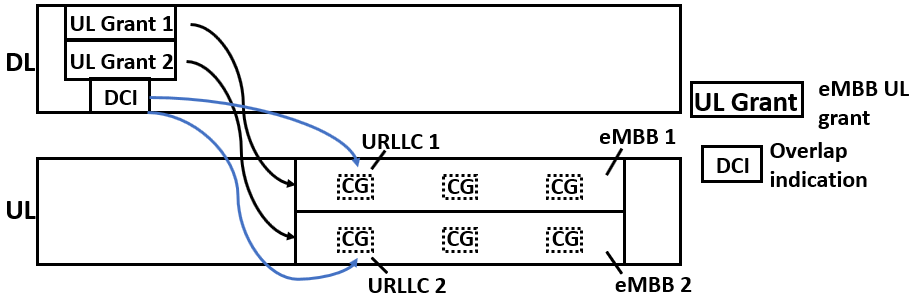
\includegraphics[scale=0.32]{fig2.PNG}}
\caption{Signalling the URLLC UEs about an overlap with the eMBB UEs in CG regions.}
\label{fig2}
\vspace{-2mm}
\end{figure}

After the URLLC UEs receive the overlap indication, the second step of the strategy starts. Thanks to the overlap indication, the URLLC UEs know about the interference and activate the explicit HARQ ACK feedback structure to replace the conventional timer-based structure. This activation can be signalled by 1-bit flag in the overlap indication. 

In this feedback structure, the UEs would be sent an ACK feedback by the gNB if data is decoded correctly at the gNB. On the other hand, if the gNB only can identify the packet by DMRS detection but cannot decode it, the UE will receive an UL grant. In the third case, if the gNB cannot identify the packet through DMRS sequence, the explicit feedback structure will help the gNB and the UE avoid packet loss. The UE does not receive ACK or UL grant from the gNB but it does not assume a successful transmission and drops data as the conventional structure. In contrast, due to a lack of feedback, the UE realizes that the gNB failed to identify its identity (ID) because of the interference between eMBB and URLLC transmission. Subsequently, the UE retransmits automatically the packet in the next available CG resources. 

Behaviors of the gNB and UE in two feedback structures are described in Table~\ref{tab1}.

\begin{table}[htbp]
\caption{Comparison of two feedback structures}
\begin{center}
\begin{tabular}{|p{8em}|p{8em}|p{8em}|}
 \hline
 \textbf{Case} & \textbf{Timer-based feedback}&\textbf{Explicit ACK feedback}\\
 \hline
 DMRS: detected&gNB: transmits no ACK/UL grant&gNB: transmits ACK\\TB: decoded &UE: considers a successful transmission &UE: considers a successful transmission\\
 \hline
  DMRS: detected&gNB: transmits UL grant &gNB: transmits UL grant\\TB: failed & UE: retransmits TB&UE: retransmits TB\\
 \hline
DMRS: failed&gNB: transmits no ACK/UL grant&gNB: transmits no ACK/UL grant\\ &UE: drops TB after time expires& UE: retransmits TB automatically after time expires\\

%  increase row height, number of & = number of collumn
% &&&&&\\[-1em]
 
 \hline
\end{tabular}
\label{tab1}
\end{center}
\vspace{-5mm}
\end{table}

%Time in the timer can be configured by radio resource control (RRC) to define how long the UE must wait for ACK or UL grant before retransmiting the packet based on reliability and latency requirements.

\subsubsection{Overlap indication and an additional SR}\label{IIB3}


An alternative technique proposed in \cite{ad99} to avoid packet loss due to DMRS miss-detection in the interference transmission is to use an overlap indication and an additional SR.

The first step is similar to the technique mentioned in Section \ref{IIB2}. An overlap indication is sent by the gNB to the URLLC UEs to inform the dynamic schedule of eMBB transmission in the CG regions.

In the second step, the overlap indication activates the URLLC UEs by 1-bit flag included in the signal to transmit an additional SR at the same time that they transmit their TBs. This SR gives the gNB another chance to identify UE ID. Indeed, if the gNB fails to detect DMRS sequence in the TB, it still can recognize the presence of the TB by decoding SR. Based on the UE ID in SR, the gNB can transmit an UL grant to reschedule a retransmission. Behaviors of the gNB and UE with the additional SR are explained in Table~\ref{tab2}.

In this scheme, the UE sends the additional SR in the dedicated PUCCH resources as illustrated in Fig.~\ref{fig3} to reduce the corruption of both DMRS detection and SR decoding because of the interference in PUSCH.

\begin{figure}[htbp]
\centerline{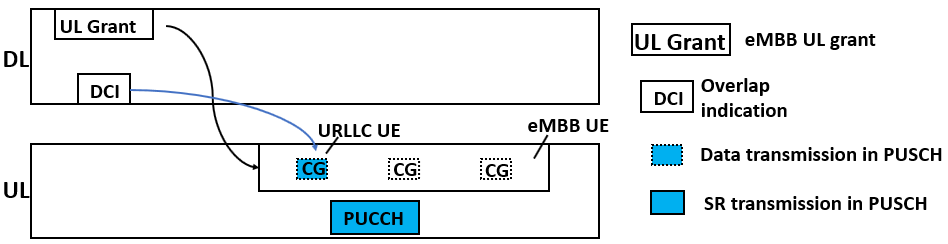
\includegraphics[scale=0.33]{fig3.PNG}}
\caption{Addition SR transmission in a dedicated PUCCH resource.}
\label{fig3}
\vspace{-2mm}
\end{figure}


The second step using explicit ACK feedback in Section \ref{IIB2} and the second step using an additional SR in Section \ref{IIB3} can be used alternatively depending on the transmission condition. The gNB chooses between two options and informs the UE by 2-bit flag in the overlap indication. Each bit is used to activate or deactivate the corresponding option. The explicit ACK feedback structure might be chosen if the period among CG occasions is small and there is no available PUCCH resource to transmit an additional SR. On the other hand, the additional SR structure is chosen if the period among CG occasions is long and latency requirement may not be satisfied with an automatic retransmission in the CG resources. 

As can be seen in Table~\ref{tab2}, the scheme with an additional SR brings benefit in case 4 when the gNB obtains the UE ID by decoding SR while failing to detect DMRS. Thereby, the gNB can sends an UL grant to reschedule a retransmission with the acquired UE ID to avoid packet loss as in the conventional scheme.  

\subsubsection{Numerical results and performance evaluation}

\begin{table}[htbp]
\caption{Simulation parameters}
\begin{center}
\begin{tabular}{|p{8em}|p{8em}|}
 \hline
 \textbf{Parameters} & \textbf{Values}\\
 \hline
 Waveform & CP-OFDM\\
 \hline
 Subcarrier spacing & 60kHz\\
 \hline
 Channel model & Rician\\
 \hline
 K factor & 1\\
 \hline
 Number of allocated PRB & 8\\
 \hline
 DMRS detection mechanism & Time-domain correlation\\
 

%  increase row height, number of & = number of collumn
% &&&&&\\[-1em]
 
 \hline
\end{tabular}
\label{tab5}
\end{center}

\end{table}

\begin{figure}[htbp]
\centerline{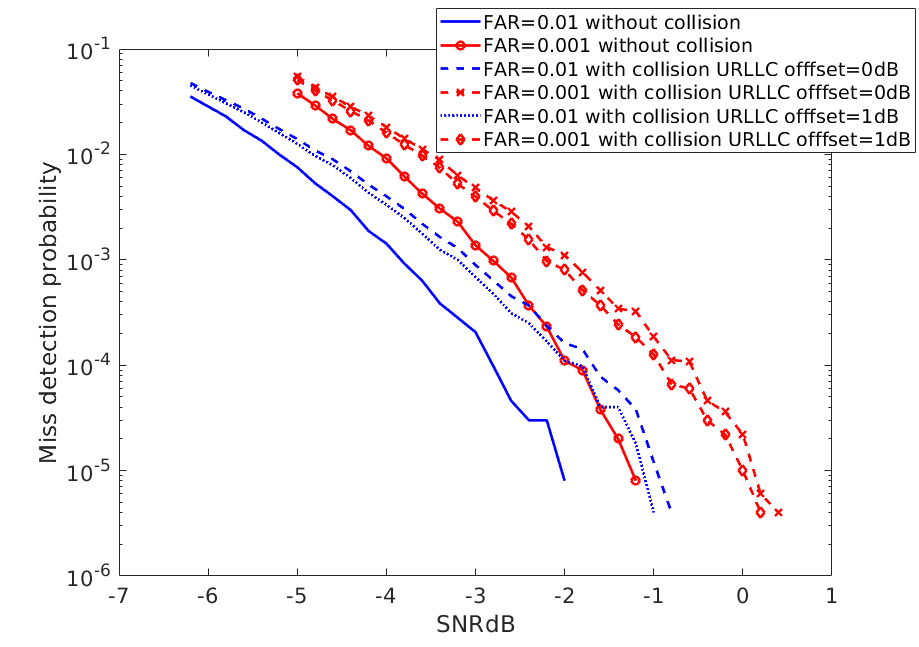
\includegraphics[scale=0.33]{fig16.png}}
\caption{DMRS detection performance.}
\label{fig16}
\vspace{-3mm}
\end{figure}

\begin{table*}[htbp]
\caption{Performance comparison between different scenarios and schemes at SNR=$-1.4dB$, FAR=0.001, $P^{e}_{d2}$=$P^{e}_{SR}$=0.01}
\begin{center}
\begin{tabular}{|p{19em}|p{9em}|p{10em}|p{12em}|}
 \hline
 \textbf{Case} & \textbf{URLLC UE ID miss detection probability}& \textbf{Retransmission in UE ID miss detection}& \textbf{URLLC UL transmission's BLER due to the first UE ID miss detection}\\
 \hline
 No collision  & 10\textsuperscript{-5}&No&10\textsuperscript{-5}\\
 \hline
 Collision in the conventional scheme& 3.4$\times$10\textsuperscript{-4}&No&3.4$\times$10\textsuperscript{-4}\\
 \hline
 Collision with power control (\cite{ref13} and \cite {ref14})&2.44$\times$10\textsuperscript{-4}&No&2.44$\times$10\textsuperscript{-4}\\
 \hline
 Collision with explicit feedback (proposed)& 3.4$\times$10\textsuperscript{-4}&Yes&3.4$\times$10\textsuperscript{-6}\\
\hline
 Collision with additional SR (proposed)& 3.4$\times$10\textsuperscript{-6}&No&3.4$\times$10\textsuperscript{-6}\\

%BLER_trans=P_DMRS+(1-P_DMRS)*P_data
%  increase row height, number of & = number of collumn
% &&&&&\\[-1em]
 
 \hline
\end{tabular}
\label{tab10}
\end{center}
\vspace{-6mm}
\end{table*}

As mentioned above, DMRS detection plays an important role in decoding and rescheduling a TB so DMRS detection performance is simulated with parameters in Table~\ref{tab5}. The simulation is done with 3 scenarios. The first scenario is when only the URLLC UE transmits data and the gNB detects DMRS sequence without any interference. The second scenario is when both the eMBB and URLLC UEs transmit in the same resource. The gNB suffers from interference when detecting DMRS sequence from the URLLC UE. The third scenario is that the URLLC UE is informed about the collision with another eMBB UE and increases power level by 1dB compared to the normal power level in case of no collision.

The gNB detects DMRS sequence by doing correlation between the received signal and the prior known sequence. The result is compared with a threshold selected based on a false alarm rate (FAR). A false alarm happens when the gNB detects a DMRS sequence whereas no actual DMRS sequence is sent. DMRS detection's performance is shown in Fig.~\ref{fig16}.

Table~\ref{tab10} shows the performance of DMRS performance at the gNB at SNR of -1.4dB, FAR of 0.001. In the conventional timer-based feedback, a DMRS miss-detection leads to a packet loss. BLER ($ P^{e}_{1}$) of the conventional timer-based feedback transmission (including the scheme of increasing power level) is 

\begin{equation}
\begin{split}
 &P^{e}_{1} = P^{e}_{DMRS1} + \\
        &+ (1-P^{e}_{DMRS1})P^{e}_{d1}(P^{e}_{DMRS2} + (1-P^{e}_{DMRS2})P^{e}_{d2}),\label{eq10}   
\end{split}
\end{equation}
where $ P^{e}_{DMRS1}, P^{e}_{DMRS2}$ are the miss detection probabilities of the initial (with collision) and retransmitted (without collision) DMRS (see Figure \ref{fig16}), and $P^{e}_{d1}, P^{e}_{d2}$ are the error probabilities of the initial (with collision) and retransmitted (without collision) PUSCH.

%In \eqref{eq10}, packet loss' probability because of DMRS miss-detection is shown in the first term. The second term is error probability when the gNB cannot decode both the initial transmission and retransmission.

When the explicit HARQ feedback structure is activated, the error probability ($ P^{e}_{2}$)  is 

\begin{equation}
\begin{split}
 &P^{e}_{2} = P^{e}_{DMRS1}(P^{e}_{DMRS2} + (1-P^{e}_{DMRS2})P^{e}_{d2}) + \\
        &+ (1-P^{e}_{DMRS1})P^{e}_{d1}(P^{e}_{DMRS2} + (1-P^{e}_{DMRS2})P^{e}_{d2}).\label{eq11}   
\end{split}
\end{equation}

$ P^{e}_{2}$ is smaller than $ P^{e}_{1}$ because the UE retransmits automatically data if it receives no ACK or UL grant as shown in the first terms of \eqref{eq10} and \eqref{eq11}. The first term $P^{e}_{DMRS1}(P^{e}_{DMRS2} + (1-P^{e}_{DMRS2})P^{e}_{d2})$ of \eqref{eq11} is smaller than the first term $P^{e}_{DMRS1}$ of \eqref{eq10} because the gNB has another chance to decode the packet if it missed DMRS sequence in the intial transmission. The numerical result in the final column of Table~\ref{tab10} shows the improvement of the DMRS miss-detection by using explicit feedback structure.

If the UE is activated to transmit an additional SR, the error probability ($ P^{e}_{3}$) is 

\begin{equation}
\begin{split}
 P^{e}_{3} &= P^{e}_{DMRS1}\times P^{e}_{SR} + \\
        &+ (1-P^{e}_{DMRS1}\times P^{e}_{SR})P^{e}_{d1}\times\\
        &\times(P^{e}_{DMRS2} + (1-P^{e}_{DMRS2})P^{e}_{d2}),\label{eq12}   
\end{split}
\end{equation}
where $P^{e}_{SR}$: the error probability of SR

The first term $P^{e}_{DMRS1}\times P^{e}_{SR}$ in \eqref{eq12} shows a decrease of error probability when the additional SR reduces DMRS miss-detection probability. The numerical result in the final column of Table~\ref{tab10} confirms the benefit of transmitting an additional SR in case of GB eMBB and CG URLLC UEs multiplexing

From the theoretical calculation in \eqref{eq10}, \eqref{eq11}, \eqref{eq12} and simulation results in Table~\ref{tab10}, the implementation of the explicit HARQ feedback structure or the transmission of a additional SR reduce the error probability due to DMRS miss-detection. The miss-detection probability increases significantly from $10^{-5}$ in non-collision case to $3.4\times10^{-4}$ in collision case that might make the URLLC transmission unable to achieve the requirements. Therefore, one of the two proposed techniques or even both two techniques at the same time in the extreme cases should be applied to guarantee the target performance.

\subsection{GB eMBB and GB URLLC multiplexing} \label{IIA}
\subsubsection{Problem formulation}\label{IIA1}

In the UL in Fig.~\ref{fig7}, when the eMBB UE has data to transmit, it sends SR to the gNB to obtain an UL grant. The gNB transmits an UL grant to allocate resources and other parameters for the eMBB UE. After the gNB schedules eMBB UL transmission, an URLLC UE also has data to transmit so it transmits SR to the gNB. Due to strict latency requirement of URLLC, the gNB must schedule the URLLC UE to the resources that are already scheduled to the eMBB UE. Therefore, there is a collision between the eMBB and URLLC UEs in those resources.

\begin{figure}[htbp]
\centerline{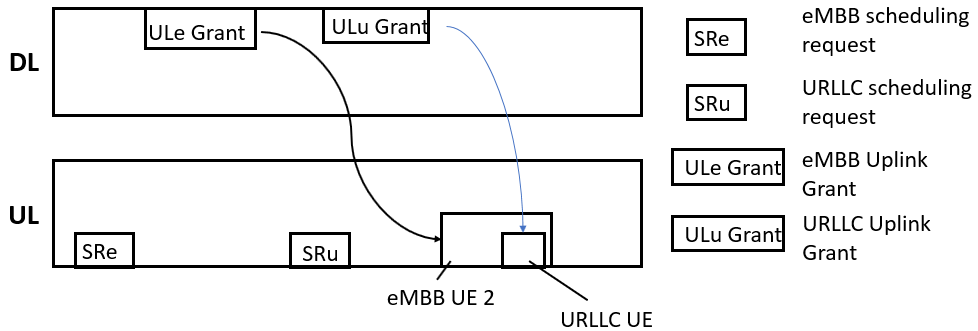
\includegraphics[scale=0.33]{fig7.PNG}}
\caption{A collision of UL URLLC GB transmission with GB eMBB transmission in case of Frequency Division Duplex (FDD).}
\label{fig7}
\vspace{-4mm}
\end{figure}

\subsubsection{Cancellation indication solution}

In \cite{ref20}, 3GPP agrees to use CI to stop the eMBB transmission in case of the collision with another URLLC GB transmission. The operation of CI is shown in Fig.~\ref{fig8}.

\begin{figure}[htbp]
\centerline{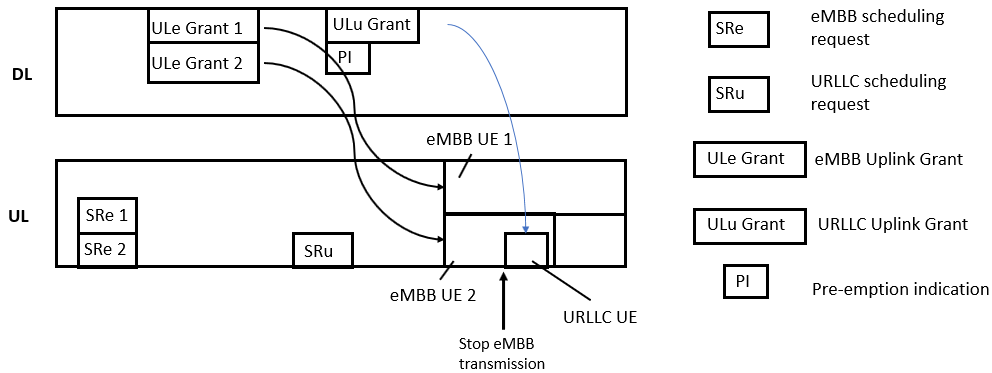
\includegraphics[scale=0.33]{fig8.PNG}}
\caption{CI transmitted to stop eMBB transmission in the region overlapping with URLLC transmission.}
\label{fig8}
\vspace{-2mm}
\end{figure}

When the gNB schedules the URLLC UE to the resources that are already allocated to the eMBB UE, it also sends CI to the eMBB UEs to stop the transmission in the overlapping resource. 3GPP supports that the transmission is stopped without resuming \cite{ref20}. 

The implementation of CI requires an enhancement of the eMBB UEs. URLLC transmission is a mini-slot transmission. Thereby, in case CI is transmitted to the eMBB UEs, it must be done on a mini-slot level to be likely to stop the transmission in time and satisfy the traffic critical delay. This design requires that the eMBB UEs monitor CI on a mini-slot level. However, the eMBB UEs transmit data on a slot level and also only monitor downlink control information (DCI) on a slot level. This means that if DCI is used as CI \cite{ref20}, the eMMB UEs are required to increase monitoring periodicity. Monitoring capability of the eMBB UEs also must be enhanced with a growth of monitoring occasions. A mechanism to select the eMBB UEs to monitor DCI on a mini-slot level and trigger an increase of monitoring periodicity and capability is still missing 3GPP Release 15. The next section describes a mechanism to fulfill those tasks. 

\subsubsection{Mechanism to activate an increase of monitoring periodicity}
When the gNB decides to allocate eMBB resources to the URLLC transmission, not all the eMBB UEs scheduled before become a candidate of the gNB's selection. One example is shown in Fig.~\ref{fig8}, the gNB chooses the eMBB UE 2 to become a candidate for a potential cancellation based on its data size. The eMBB UE 2 has a smaller packet than the eMBB UE 1 so the gNB consumes less resources for a retransmission after cancelling its transmission. 

For this reason, only the eMBB UE 2 that has been chosen by the gNB for a potential data cancellation. Thus, only this UE has to increase its monitoring periodicity for CI monitoring in mini-slot level. The gNB triggers this increase when it chooses the eMBB UE candidates for cancellation.

Another way to choose the UE candidates is based on the UE capability. Not all eMBB UEs are able to listen to DCI in mini-slot so these UEs are not chosen to stop the transmission in the overlapping region because it might not be likely to stop the transmission in short delay to satisfy URLLC latency requirement.
The positions of the eMBB UEs are also taken into account. The UEs at the edge of cell are not chosen for potential cancellation because these UEs use higher power and lower MCS for the initial transmission to achieve the requirement so much more power and resources are needed for a retransmission than the UEs being near to the gNB. Channel condition that the gNB knows from SR is also a criterion to choose UE candidate for cancellation.

The eMBB UE candidates are chosen based on selection criteria following the order: UE capability, UE position to the gNB, data size and channel condition. The basic idea here is that the gNB can apply some selection rules on the transmissions to limit the eMBB UEs that might be pre-empted.

If the eMBB UEs are configured to monitor CI in mini-slot level all the time after being scheduled, power consumption would rise significantly. Therefore, only the eMBB UEs chosen based on the criteria mentioned above are triggered to increase monitoring periodicity. This activation is done by the gNB using 1-bit flag in the UL grant for the eMBB UEs to help them perceive their situation and do monitoring in mini-slot level as shown in Fig.~\ref{fig17}. The bit used as a flag can be a padding bit or the first bit in the field of frequency domain resource assignment in DCI used as UL grant.

\begin{figure}[htbp]
\centerline{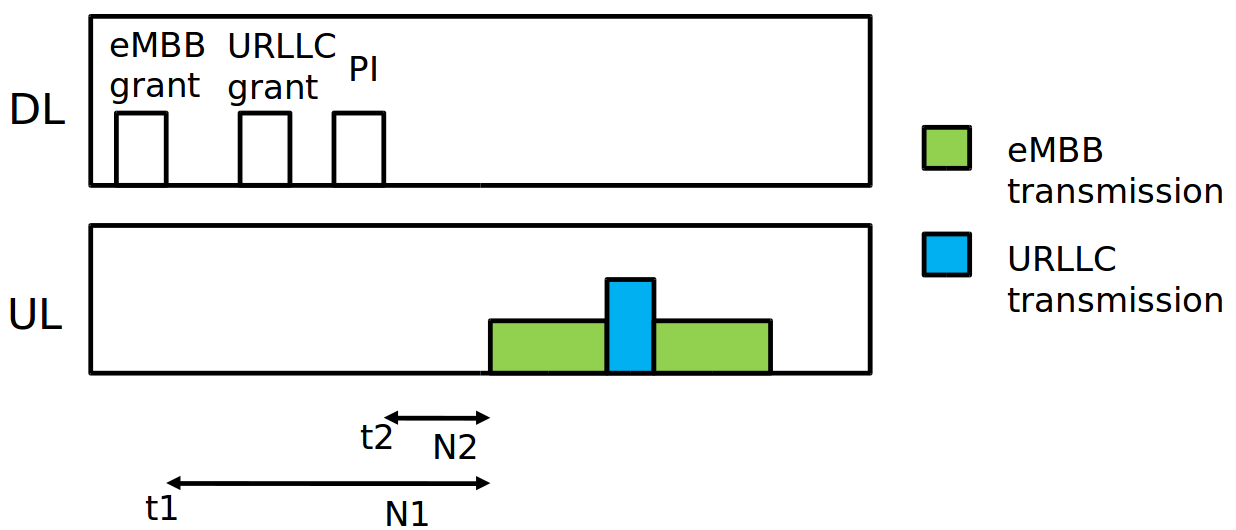
\includegraphics[scale=0.17]{fig17.png}}
\caption{Activating timing of CI.}
\label{fig17}
\vspace{-2mm}
\end{figure}

Another option to implement 1-bit flag without increasing payload of UL grant is to embed the flag signal in DMRS. Two phase shifted versions of the same DMRS base sequence are used for UL grant. The phase shift value is 90 degree to create two orthogonal versions. One version is to indicate that the eMBB UE is not a candidate to monitor CI in mini-slot level. The other version is to indicate that the eMBB UE might have to stop its transmission and needs to monitor CI in mini-slot level. 

The eMBB UE does not need to increase monitoring periodicity and listen to CI immediately after receiving 1-bit flag in UL grant. As illustrated in Fig.~\ref{fig17}, the eMBB UE does not need to increase monitoring periodicity at $t_1$ because its transmission still have not started. The gNB only starts to transmit CI after $t_2$. The moment $t_2$ is chosen based on the processing capability $N_2$ of the eMBB UE. It is to ensure that the eMBB UE can decode CI before its transmission. This means that the eMBB UE only needs to increase monitoring periodicity and listen to CI after $t_2$. It helps the UE save energy in the interval of $N_1-N_2$.

If an eMBB UE receives a positive flag from the gNB in the UL grant, it will increase the monitoring periodicity from slot level to mini-slot level. An increase of monitoring periodicity can be carried out without a big modification in the UE design. In 5G NR, the UE supports different SCS: 15 kHz, 30 kHz, 60 kHz, 120 kHz. 

\begin{figure}[htbp]
\centerline{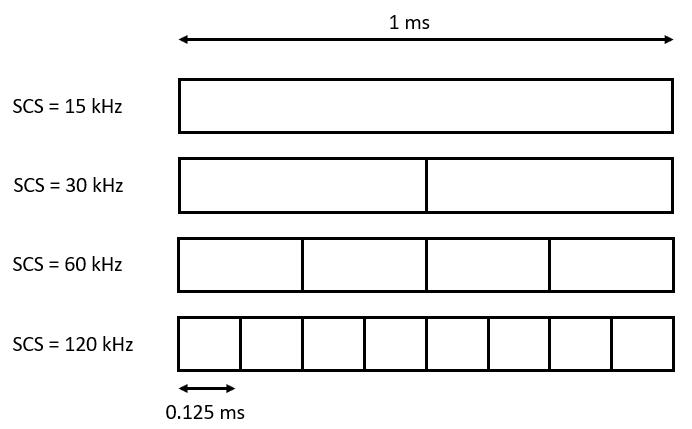
\includegraphics[scale=0.3]{fig9.PNG}}
\caption{SCS terminology.}
\label{fig9}
\vspace{-6mm}
\end{figure}

In 1 ms, the maximum number of slots are 8 slots with SCS of 120 kHz. If the UEs monitor DCI in slot level, they have 8 monitoring occasions. This means that the UEs are already capable of supporting 8 monitoring occasions with their current design. Therefore, it is proposed that the number of monitoring occasions are still kept the same at 8 occasions in 1 ms even if the value of SCS decreases after the eMBB UEs receive 1-bit flag in UL grant. This value allows the eMBB UEs to monitor CI in mini-slot level when a low SCS is used. Normally, with SCS 60 kHz, there are only 4 monitoring occasions in 1 ms. However, with this proposal, the number of occasions are doubled to 8. At this moment, the UEs monitor DCI in non-slot level at each interval of 0.125 ms. The impact of this proposal is even bigger for low SCS 15 kHz and 30 kHz. In general, when an eMBB UE is indicated to decode CI in sub-slot level, it can be configured to DCI periodicity going up to its highest capability sub-carrier spacing slot timing. 

Monitoring capability also have to be enhanced if monitoring occasions increases, especially for SCS 15 kHz. In normal case, the UEs have 44 PDCCH candidates and 56 non-overlapped CCEs in a 1ms-slot with SCS 15 kHz. When the number of occasions grow to 8 in 1ms-slot, the UEs only have around 5 PDCCH candidates and 7 CCEs for each monitoring occasion. If an aggregation level (AL) 8 is required for CI so as to guarantee the reliability, there are not enough CCEs for that CI. Due to the very high reliability of URLLC transmission, the reliability of CI to stop the eMBB transmission needs to be approximately the same as the one for URLLC (10\textsuperscript{-5}). The maximum number of CCEs should be kept the same at 64 CCEs for all SCS to ensure that CI is bound to be transmitted with AL 8. Similar to the proposal of the value of monitoring occasions, this maximum number of CCEs are only applied after the eMBB UEs receive an indication of 1 bit-flag in UL grant.

\subsubsection{Period of monitoring occasion}
URLLC transmission is carried out in mini-slot level with period of 2, 4 and 7 symbols for normal prefix or 2, 4, 6 symbols for extended prefix. The eMBB UEs are required to monitor CI in the same period of URLLC transmission so they can realize the overlapping situation indicated by the gNB and stop their transmission in the shortest delay. This means that monitoring occasions increase from 1 per slot to 7, 4 and 2 corresponding to period of 2, 4 and 7 symbols of URLLC transmission for normal prefix or 7, 4 and 3 corresponding to period of 2, 4 and 6 symbols of URLLC transmission for extended prefix. The requirement of monitoring periodicity can be relaxed and larger than the scheduling transmission level of URLLC if the traffic is not much sensitive to latency. 

\subsubsection {CI design}

DCI used for UL CI is encoded and transmitted on PDCCH. There are two options to transmit DCI containing CI: GC CI and UE-specific CI.

\begin{figure}[htbp]
\centerline{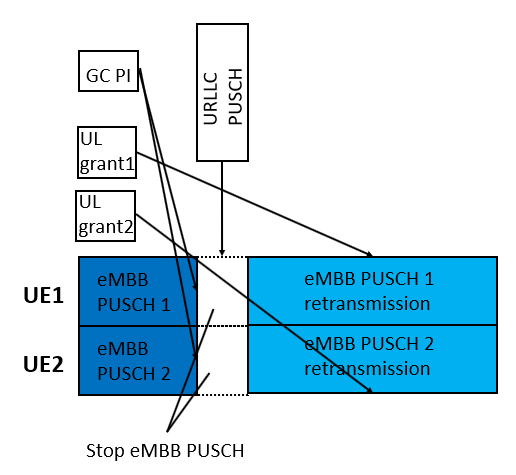
\includegraphics[scale=0.38]{fig10.PNG}}
\caption{GC CI operation to stop eMBB transmission in the overlapping region.}
\label{fig10}
\vspace{-2mm}
\end{figure}

The operation of GC CI is shown in Fig.~\ref{fig10}. A GC CI is transmitted by the gNB to all the eMBB UEs in its coverage. Reliability of this CI is equivalent to the URLLC reliability requirement (10\textsuperscript{-5}) because if the eMBB transmissions do not stop in time, they will affect the performance of the URLLC transmission. The GC CI indicates the exact time and frequency of the overlapping URLLC resources. After decoding GC CI, the eMBB UEs who realize an overlap stop their ongoing transmissions without resuming. The URLLC UE, thus, can transmit in the collision-free resource. Consequently, the gNB must reschedule the retransmissions for the eMBB UEs stopping their ongoing transmissions. The gNB sends UE specific UL grants to the eMBB UEs. These UL grants is only required to achieve eMBB reliability (10\textsuperscript{-2}).

\begin{figure}[htbp]
\centerline{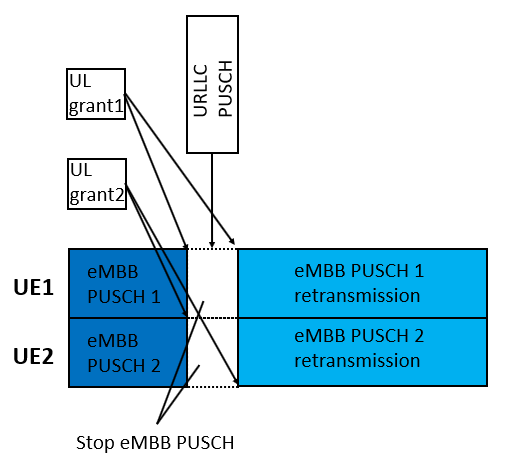
\includegraphics[scale=0.4]{fig11.PNG}}
\caption{UE-specific CI operation to stop eMBB transmission in the overlapping region.}
\label{fig11}
\vspace{-2mm}
\end{figure}

The operation of UE-specific CI is shown in Fig.~\ref{fig11}. This UE-specific CI has two roles. The first one is to stop the eMBB transmissions that are overlapped by the URLLC transmission. The second one is to reschedule the eMBB transmissions that are cancelled. The UE-specific CI has the same format as legacy UL grants. It contains the same HARQ process of the ongoing transmission. Therefore, if the eMBB UE having an ongoing transmission receives such CI (UL grant), it interprets that signal as UL cancellation and rescheduling. The resources for the retransmission are indicated by the UE-specific CI. The eMBB UEs stop their transmission as soon as the correct decoding of CI. The UE-specific CI is required to have the URLLC reliability to guarantee no interference from the eMBB transmission to the URLLC transmission.

DL resource consumption can be optimized by selecting between GC CI and UE-specific CI based on the number of the overlapping eMBB UEs.

We assume that $N$ eMBB UEs have the ongoing transmissions overlapped by the URLLC UE at a specific moment. 

If GC CI is used, one GC CI and $N$ rescheduling UL grants are needed in the process. The aggregation level (AL) of GC CI achieves URLLC reliability requirement is: $R_{1}$. Rescheduling UL grant with eMBB reliability requirement is configured with a lower AL: $R_{2}$. The total ALs in the process are: $R_{1} + R_{2}\times N$.

If UE-specific CI is used, $N$ UE-specific CIs are transmitted to stop the ongoing transmissions and schedules the retransmissions. Each UE-specific CI must achieve URLLC reliability requirement with AL: $R_{3}$. The total ALs in the process are: $R_{3}\times N$.

In one scenario, $R_{1}$ must guarantee URLLC reliability requirement for all the eMBB UEs with different locations and channel condition so a large AL of $R_{1}$ equal to 8 is required. The rescheduling UL grant transmitted after GC CI only needs to attain eMBB reliability requirement so a small AL of $R_{2}$ equal to 2 is used. For the combining of CI and UL grant in the UE-specific CI, this CI must achieve URLLC reliability requirement only for the target eMBB UE so an AL of $R_{3}$ equal to 4 is used. In this case, if the number of the eMBB UEs are smaller than 4, the UE-specific CI is used because of less resource consumption. On the other hand, if the eMBB UEs are bigger than 4, the GC CI is used.

At the time, the gNB schedules URLLC transmission, it calculates the resource consumption in DL with CI and UL grant to decide to choose GC or UE-specific CI. A flexible scheme in using CI helps to optimize resource consumption.

Due to high reliability requirements of CI, high Als are used for CI. Thus, when the eMBB UEs are triggered to monitor CI on mini-slot level by an active flag, they only search for PDCCH candidates with high ALs in the search space instead of searching from the smallest AL to the biggest AL as conventional. In the common search space, the eMBB UEs search the PDCCH candidates with AL 8 and 16 to find GC CI. In UE search space, the eMBB UEs search the PDCCH candidates with AL 4 and 8 to find UE-specific CI. This constraint reduces the number of blind decodes and energy consumption of the UEs.

\section{Ensuring Latency and Reliability with UL Configured Grant transmissions}\label{III}
\subsection{Problem formulation}

3GPP Release 15 enhances URLLC reliability and latency by standardizing that the UEs can transmit automatically $K$ repetitions without waiting feedback from the gNB in the CG resources as configured by parameter $repK$ from higher layer. The values of $K$ are 1, 2, 4 and 8 \cite{ref6}.

The standard puts a constraint to the automatic repetitions of UL packets. The UEs are only allowed to carry out repetitions of a packet in an interval with periodicity $P$. The range of $P$ is from several symbols to several slots as standardized in \cite{ref6}. In case the UE reaches the boundary of an interval, it must stop the repetitions of the corresponding packet starting in that interval even if the maximum number of repetitions have not been attained. This constraint is to avoid a confusion of HARQ IDs of the repetitions in different HARQ process at the gNB. If the gNB misses the first transmission then the second and third transmissions have different IDs, the gNB will not know the ID of the original transmission to send an UL grant for a retransmission. Moreover, the gNB also cannot recognize the order of the repetitions to do soft combining in that scenario. 

Due to the constraint of interval boundary, the number of repetitions transmitted might be smaller than the configured number $K$ as shown in Fig.~\ref{fig4} where $K$ is configured to 4. An interval of a HARQ process with time length $P$ contains 4 CG occasions. For the first packet, it arrives at the beginning of an interval and before all 4 CG occasions so the UE can carry out 4 repetitions as configured. Nevertheless, the second and third packet comes after the first CG occasion, thus, the UE is only able to do 3 and 2 repetitions, respectively, instead of 4 repetitions as configured. 

\begin{figure}[htbp]
\centerline{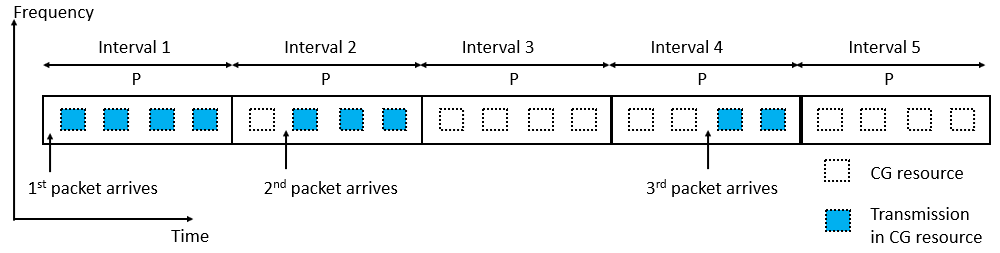
\includegraphics[scale=0.33]{fig4.PNG}}
\caption{Less than K repetitions in CG UL transmission.}
\label{fig4}
\vspace{-3mm}
\end{figure}

Reliability of UL CG transmission decreases when the number of actual repetitions are smaller than the configured number. This situation also increases latency of the transmission because the gNB would need to reschedule the packet and waits for the next round of retransmission to decode the packet. This amount of time might be larger than the URLLC latency target.

\subsection{Prior art}\label{IIIBN}
In 3GPP Release 15, the UE only can wait until the next interval to transmit all $K$ repetitions if data arrives lately. The waiting time might be large if SCS is small or the packet arrives only after some CG occasions as the second packet in Fig.~\ref{fig4}. Latency requirement may not be satisfied in those cases.

In \cite{ref7}, 3GPP agreed that multiple configurations are used to enhance reliability and reduce latency. Ensuring $K$ repetitions is included in the goal of multiple configurations. The UE can choose the configuration with the closest starting point to transmit all $K$ repetitions as shown in Fig.~\ref{fig14}. Two drawbacks of this scheme are overhead of signal to schedule multiple configurations and resource consumption of multiple configurations. For this reason, the main motivation for multiple configuration is for different applications with different requirements.

\begin{figure}[htbp]
\centerline{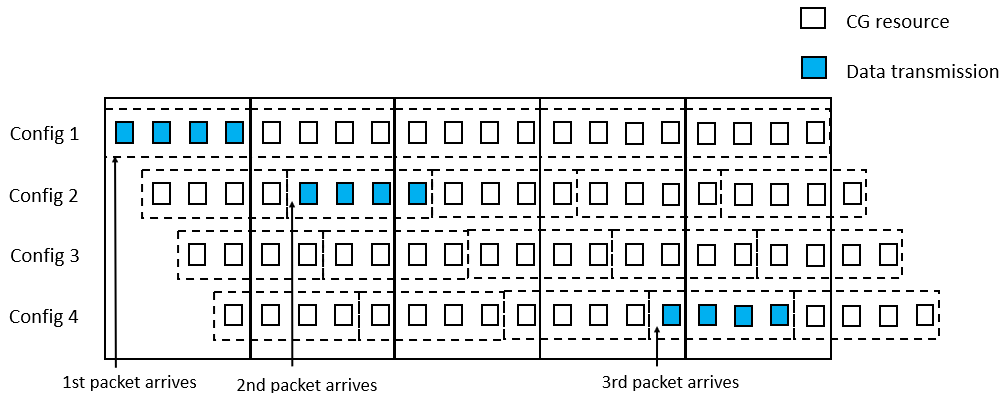
\includegraphics[scale=0.32]{fig14.PNG}}
\caption{Multiple configurations to ensure $K$ repetitions.}
\label{fig14}
\vspace{-4mm}
\end{figure}


In \cite{ref8} and \cite{ref9}, the UE is able to transmit the repetitions across the consecutive HARQ interval. It requires lots of effort in standardization to avoid the confusion between HARQ IDs at the gNB such as a mechanism to communicate HARQ IDs to the gNB or different DMRS sequences in the repetitions.

In \cite{ref10} and \cite{ref11}, the UEs transmits the repetitions in the shared resource. However, the constraint of HARQ process boundary is not considered. Moreover, the size of all resources for repetitions are the same. Both factors cause a degradation of reliability, latency and resource consumption.

\subsection{Optimal reserved resources to ensure $K$ repetitions}\label{IIIB}

\subsubsection {Reserved resources}

For CG transmission, each interval is associated with a HARQ process and that's why a TB is not allowed to cross the boundary of an interval. The configured number of repetitions can be guaranteed by generating some transmission resources which are dedicated for the CG transmissions in case the repetitions can not be completed within the classic resources as we propose in \cite{b9}. The reserved resources are configured with the same period as CG occasions. These reserved resources are shared shared among the UEs following random access or group access, resulting in lower overhead of resource creation. If the UE reaches the boundary of a HARQ process while not carrying out $K$ repetitions, it will use the reserved resources configured in the next transmission interval (reserved for a different HARQ process) to continue to transmit until attaining $K$ repetitions as shown in Fig.~\ref{fig5}. Due to the boundary of the first period, the UE1 only transmits 3 repetitions but continues to transmit 1 repetition remaining in the first reserved resource of the next period instead of stopping the transmission. The gNB will search the reserved resources to find the repetitions. Because the reserved resources are configured by the gNB, it can distinguish the repetitions in the CG and reserved resources. Therefore, the gNB only uses HARQ ID of repetitions in the CG resource for UL grant for a retransmission.

\begin{figure}[htbp]
\centerline{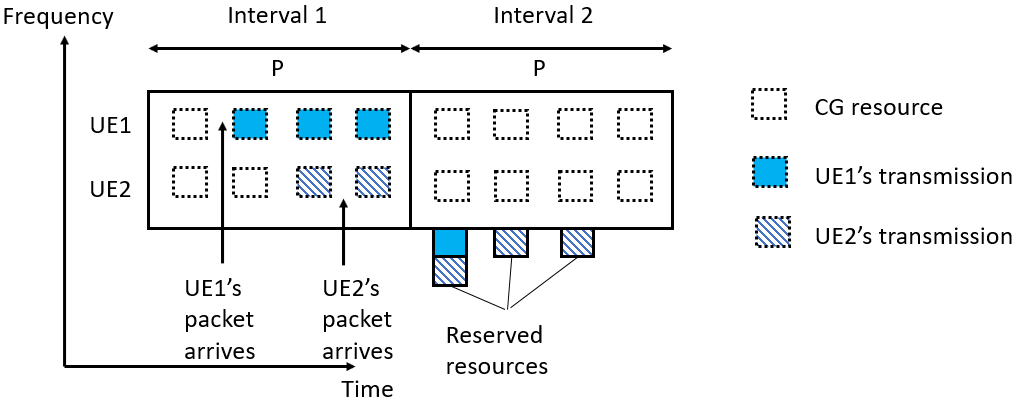
\includegraphics[scale=0.32]{fig5.PNG}}
\caption{Reserved resources for repetitions.}
\label{fig5}
\vspace{-2mm}
\end{figure}

\subsubsection{System model} \label{IIIB2}

\begin{figure}[htbp]
\centerline{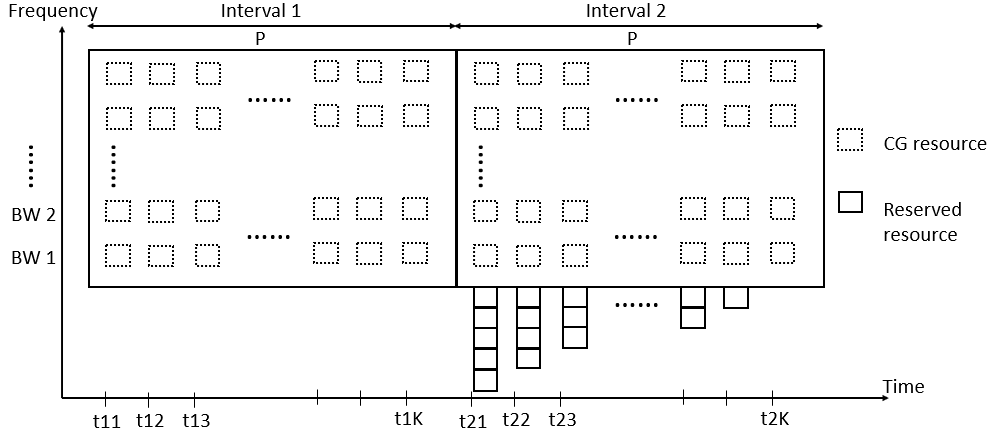
\includegraphics[scale=0.33]{fig6.PNG}}
\caption{UL transmission resources' distribution.}
\label{fig6}
\vspace{-2mm}
\end{figure}



In Fig.~\ref{fig6}, there are $N$ UEs configured to transmit $K$ repetitions in the contiguous CG resources. The CG resources in one frequency band can be shared among the UEs in a group. A HARQ process with time interval $P$ contains $K$ CG transmission occasions. The results derived below are also valid if the number of CG transmission occasions in an interval $P$ are bigger than $K$. $K-1$ reserved resources are configured with the same period as the CG resources in each period $P$. All $N$ UEs can use the reserved resources to attain the configured number of repetitions. Each reserved resource has size of $M_{i}$ blocks where each block has the size of CG resource in one transmission occasion with index $i$ indicating that the reserved resource is at the $i$th transmission occasion of a period. 

The arrival of data for each UE follows a Poisson process with the average number of random access events in an interval $\lambda$ calculated from the period between the CG resources $T$ and an average packet inter-arrival time $\mu$: $\lambda$ = $T/\mu$.

\subsubsection{Collision probability in reserved resources}\label{IIIB3}

With random access, the $N$ UEs in system are allowed to use any block in the reserved resources of a specific transmission occasion if they need to do the transmissions in order to fulfill the configured number of repetitions.

The collision probability in the reserved resource at the first transmission occasion of a period (at t21 in Fig.~\ref{fig6}) is calculated as follow by considering 1 UE of interest having a transmission in the reserved resource at t21 and the rest of $N-1$ UEs.

It is assumed that the packet of the UE of interest cannot be decoded by the gNB if there is a collision with packets of other UEs in the reserved resources. The calculations below only focus on the error due to collision and do not count the radio errors.

In time $T$ between two CG resources, the probability that one UE has one or more random transmissions is

\begin{equation}
P_{data} = 1 - e^{-\lambda},\label{eq1}
\end{equation}

The CG resources in one bandwidth can be shared between a group of the UEs so collision probability in the CG resources between the UE of interest and other UEs of group is 

\begin{equation}
P_{c\_CG} = 1 - e^{-\lambda(N_\mathrm{UE\_group}-1)},\label{eq2}
\end{equation}
where $N_\mathrm{UE\_group}$ is the number of the UEs that use the same frequency band of CG resources.

The reserved resource at t21 is used by a UE if its data comes after the first CG transmission occasion at t11. The probability that one UE has transmission after the first CG transmission occasion in a period $P$ is 

\begin{equation}
P_{d} = 1 - (1-P_{data})^{K-1}.\label{eq3}
\end{equation}

There is no collision in the first reserved resource of a period $P$ at t21 if no UE rather than the UE of interest has a transmission after the first CG transmission occasion at t11. The probability that no other UE from the set of $N-1$ UEs has a transmission after the first CG occasion is calculated by 

\begin{equation}
P_{0} = (1-P_{d})^{N-1}.\label{eq4}
\end{equation}

In case other UEs in a set of $N-1$ UEs has a transmission after the first CG occasion, the probability that $n$  UEs have such transmission is 

\begin{equation}
P_{n} = \binom {N-1}{n}P_{d}^{n}(1-P_{d})^{N-1-n}.\label{eq5}
\end{equation}

The probability that the UE of interest and $n$ UEs do not access the same resource block in the first reserved resource at t21 is 

\begin{equation}
P_{a0\_n} = \left(\frac {M_{1}-1}{M_{1}}\right)^{n}.\label{eq6}
\end{equation}

The probability that the UE of interest does not collide with any other UE in the first reserved resource at t21 is calculated by 

\begin{equation}
P_{sum} = \sum_{n=1}^{N-1} P_{n}P_{a0\_n}.\label{eq7}
\end{equation}

From \eqref{eq4} and \eqref{eq7}, the collision probability in the first reserved resource for the UE of interest is derived as 

\begin{align}
P_{c1} &= 1 - P_{0} - P_{sum} \nonumber\\
 &= 1 - \left(\frac{M_{1}-1+e^{-\lambda(K-1)}}{M_{1}}\right)^{N-1}.\label{eq8}
\end{align}

Based on the same calculating process, a general equation of collision probability for the reserved resource at any transmission occasion in a period can be derived as 

\begin{equation}
P_{ci} = 1 - \left(\frac{M_{i}-1+e^{-\lambda(K-i)}}{M_{i}}\right)^{N-1},\label{eq9}
\end{equation}
where
$i \in [1, K-1]$ is index indicating the position of the reserved resource based on the position of transmission occasion in a period.

According to \eqref{eq9}, if $P_{ci}$ is set to have the same value in all the reserved resources, the sizes of the reserved resources in an interval decrease from the first one to the last one: $M_1 > M_2 > M_3 > ... > M_{K-1}$. This means that the sizes of the reserved resources are optimized based on their positions. This optimization reduces resource consumption compared to using the same size for all reserved resources.

\subsubsection{SIC receiver at the gNB}

The technique that we proposed in \cite{b9} is developed further in this section. In the calculation in Section \ref{IIIB3}, a packet is assumed not to be decoded if it collides with the packets of other UEs in the reserved resources. However, even if there is a collision between the repetitions of the UEs in the system, the gNB equipped with a SIC receiver still can decode correctly the repetitions. When the gNB decodes correctly a packet in the CG resources or the previous reserved resources, it stores that packet. After that, if the gNB encounters a collision between the successful packet and another packet in the reserved resources, it can cancel the successful packet from the received signal to remove the interference. Thereby, the gNB decodes the other packet without interference and has higher successful probability. With big number of repetitions (for example, 4 or  8 repetitions), there is low probability that the gNB has a collision among all non-decoded packets so the SIC receiver is useful in improving performance of repetitions in the reserved resources.

The successful probability of a packet in the transmission with SIC receiver in the gNB is complex to calculate. It depends on the channel condition of other UEs, the successful probability of other packets competing for the resources, the time arrival of data. Therefore,a model of SIC receiver in physical layer called K-multipacket reception (K-MPR) is used in \cite{ref21}. In this model, the gNB is assumed to be able to decode correctly all the UE transmissions in the same block of reserved resources if the number of the UEs in that block are smaller than a threshold $L$. On the contrary, if the number of the collided UEs are bigger than $L$, all the packets in the collided resources cannot be decoded.

Using the system model in \ref{IIIB2}, the equations calculated in \ref{IIIB3} and the model of SIC receiver in \cite{ref21} , the error probability of a packet due to the collision is calculated for the first reserved resource at t21 in Fig.~\ref{fig6}. We consider a UE of interest and other $N-1$ UEs.

The probability that n UEs in $N-1$ UEs have a transmission is calculated in \eqref{eq5}. The probability that $l$ UEs in these $n$ UEs access the same block in the first reserved resource as the UE of interest is

\begin{equation}
P_{al\_n} = \binom {n}{l}\left(\frac{1}{M_{1}}\right)^{l}
\left(\frac {M_{1}-1}{M_{1}}\right)^{n-l}.\label{eq13}
\end{equation}

If the value of $l$ is smaller than $L-1$, the gNB still can decode all the packets in that block. The probability that the UE of interest collides with any other UEs ($l<L-1$) but the packet is still decodable in one block is

\begin{align}
P_{s} &= \sum_{n=1}^{N-1} P_{n}\sum_{l=1}^{L-1}P_{al\_n} \nonumber\\
 &= \sum_{n=1}^{N-1} P_{n}\sum_{l=1}^{L-1}\binom {n}{l}\left(\frac{1}{M_{1}}\right)^{l}
\left(\frac {M_{1}-1}{M_{1}}\right)^{n-l}.\label{eq14}
\end{align}

From \eqref{eq4}, \eqref{eq7} and \eqref{eq14}, the error probability of a packet from the UE of interest due to collision in the first reserved resource is

\begin{align}
P_{col\_SIC\_1} &= 1 - P_{0} - P_{sum} - P_{s} \nonumber\\
 &= 1- (1-P_{d})^{N-1} - \nonumber\\
 &- \sum_{n=1}^{N-1} P_{n}\sum_{l=0}^{L-1}\binom {n}{l}\left(\frac{1}{M_{1}}\right)^{l}
\left(\frac {M_{1}-1}{M_{1}}\right)^{n-l}.\label{eq15}
\end{align}

\eqref{eq8} is a case of \eqref{eq15} where $L$ is 1 and the packet cannot be decoded if there is a collision. 

The presence of SIC receiver reduces resource consumption of the reserved resources, make the system support more UEs with higher data arrival rate.

\subsection{Explicit HARQ feedback structure to reduce packet loss in less than K-repetition situation}\label{IIIC}

In case the PUSCH resources for UL transmission is scarce and the network is overloaded with the UEs, the gNB cannot configure reserved resources to guarantee both the number of repetitions and their reliability. The network faces the fact that the number of repetitions are impossible to be achieved as configured. The priority in this situation is to reduce the impact of the repetitions that are not transmitted to system's reliability. The schemes described Section in \ref{IIIC} and Section \ref{IIID} will attain this goal.

When the gNB configures $K$ repetitions to an UL CG transmission, it calculates and sets up all parameter to make sure that the system achieves the target reliability in a channel condition. If the UEs transmits less than $K$ repetitions due to the constraint of interval boundary, it makes the system operate under target operation point. Thereby, error probability including DMRS miss-detection becomes bigger. Normally, if the gNB identifies a packet but cannot decode it, it can reschedule a retransmission. But if it misses DMRS of the packet, it cannot reschedule the packet. The packet is just dropped by the UE because of timer-based feedback structure as explained in Section \ref{IIB1}. To avoid this outcome and improve reliability, we propose in \cite{ad100} a strategy related to the activation of explicit HARQ ACK feedback structure as in Section \ref{IIB2}.

When the UE transmits a packet less than $K$ repetitions, the explicit HARQ ACK feedback structure is activated for that packet. The UE expects ACK from the gNB in case of a successful transmission instead of no feedback. The gNB also recognizes the smaller number of repetitions received by counting the repetitions in the prior known interval with period $P$. Consequently, the gNB knows that an explicit feedback structure is used. It transmits ACK to the UE if it decodes correctly one of the repetitions of the concerned packet.

The explicit HARQ feedback structure is only activated in the extreme cases as less-than-K-repetition transmission when the probability of DMRS detection becomes high. Another case is when there is an interference between eMBB and URLLC transmission described in Section \ref{IIB2}. The selective activation of the explicit feedback structure helps to increase the system's performance in the extreme case while does not increase the overhead of ACK feedback in the normal cases. In those cases, reliability of URLLC transmission is ultra high so an ACK feedback is not necessary and only wastes resource.

In the explicit HARQ feedback structure, the UE receives ACK if the packet is decoded and UL grant if only DMRS of the packet is detected. If the UE receives no feedback, the UE knows that the gNB misses UE ID and retransmits automatically data in the CG occasions.

The explicit feedback might be combined with the strategy of using reserved resources in Section \ref{IIIB}. An explicit HARQ-ACK feedback is expected from the gNB to prevent the UEs from doing the unnecessary transmissions in the reserved resources. It helps to avoid that the redundant data transmitted might cause a collision with data of other UEs that really need to be transmitted in the reserved resource to achieve reliability requirement. The presence of an explicit ACK feedback reduces resource consumption for retransmissions, the sizes of the reserved resources as well as increases reliability of the transmission. 

\subsection{Additional SR to reduce packet loss in less than K-repetition situation}\label{IIID}

An alternative scheme that we propose in \cite{ad100} can be used to improved the probability of UE ID detection if the UEs transmit less than $K$ repetitions. An additional SR is transmitted in parallel with data if the UE realizes that it is only able to carry out less than $K$ repetitions of the packet. SR is transmitted in the dedicated PUCCH separated from PUSCH to provide another mean for the gNB to identify UE ID.

Behaviors of the gNB and UE with the additional SR are summarized in Table~\ref{tab2} of Section \ref{IIB3}. 

Both two strategies in \ref{IIIC} and \ref{IIID} can be activated at the same time in case of less-than-K-repetition transmission if the URLLC requirements are very strict.

\subsection{Numerical results and performance evaluation}\label{IV}

\subsubsection{Optimal reserved resources}
\paragraph{No SIC receiver at the gNB}\label{IVB1}
In the first scenario, the set of the parameters is: $M_1=10, K=4, \lambda=1.25\times10^{-4}, P_{c1}=10^{-3}$.  This means that the UEs are configured to transmit 4 repetitions. The size of the first reserved resources is 10 blocks. The goal is to find the maximum number of the UEs with a collision probability in the reserved resource of 10\textsuperscript{-3}. The collision probability with respect to the number of the UEs sharing the reserved resources is illustrated in Fig.~\ref{fig12}. As can be seen in the graph, the system can support 28 UEs in the first reserved resources.

\begin{figure}[htbp]
\centerline{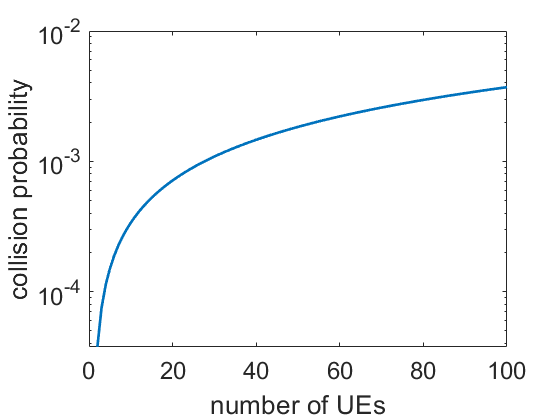
\includegraphics[scale=0.35]{fig12.png}}
\caption{Collision probability with respect to the number of the UEs.}
\vspace{-2mm}
\label{fig12}

\end{figure}


In \eqref{eq2}, it is mentioned that the UEs share not only the reserved resources but also the CG resources. 28 UEs are divided into the groups that the UEs in each group share the CG resources in one bandwidth. The collision probability calculated from \eqref{eq2} is set to be approximate to the target probability $P_{c1}=10^{-3}$. Therefore, 28 UEs are divided into 4 groups with 7 UEs in each group. $P_{c\_CG}$ in \eqref{eq2} is $7.5\times10^{-4}$.


After finding the number of the UEs in the system, the next step is to find the optimal size of the second and the third resources with the same set of the parameters. Because 4 repetitions are configured, 3 reserved resources in 3 consecutive locations of the next period are required. The reserved resources' optimal sizes are shown in Table~\ref{tab3}.
%Fig.~\ref{fig13} shows collision probability with respect to the size of the second reserved resource. The optimal size of the second reserved resource to achieve $P_{c1} = P_{c2} = 10^{-3}$ is 7 blocks.

%\begin{figure}[htbp]
%\centerline{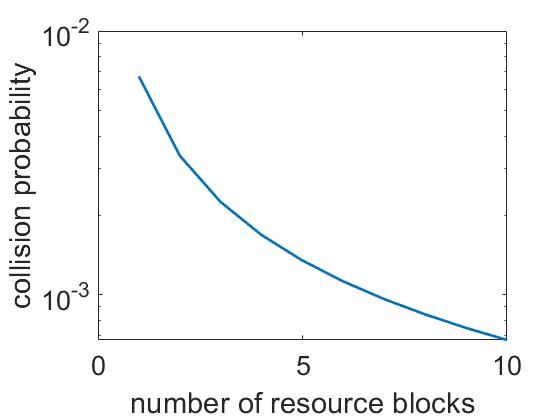
\includegraphics[scale=0.35]{fig13.png}}
%\caption{Collision probability in the second reserved resource.}
%\vspace{-2mm}
%\label{fig13}

%\end{figure}



\begin{table}[htbp]
\caption{Sizes of the reserved resources with $K=4$ and random access}
\begin{center}
\begin{tabular}{|p{10em}|p{2em}|p{2em}|p{2em}|}
 \hline
 \textbf{\textit{Position of reserved resources}} & $1$ &$2$ &$3$ \\ 
 \hline
 \textbf{\textit{Number of blocks}} & $10$ &$7$ &$3$ \\

%  increase row height, number of & = number of collumn
% &&&&&\\[-1em]
 
 \hline
\end{tabular}
\label{tab3}
\vspace{-2mm}
\end{center}

\end{table}

In comparison to the scheme that the sizes of all reserved resources are equal as in \cite{ref10} and \cite{ref11}, the proposed scheme with reserved resources helps to reduce resource consumption by $(1 - (10+7+3)/(10\times3))\times100\% = 33\%$.

The proposed scheme also consumes much less resources than the scheme of multiple configurations in  \cite{ref7}. As shown in Fig.~\ref{fig14}, if 4 repetitions are configured by the gNB, 4 configurations must be configured to ensure that the UEs always can transmit at the beginning of a period and reach 4 repetitions as configured. For a group of the UEs sharing the CG resources, 4 configurations are needed. Each configuration consists of 4 CG resources in one period. Thus, one group of the UEs requires $4\times4 = 16$ resource blocks in a period. As mentioned in the first scenario, there are 4 groups of the UE so in total, $16\times4 = 64$ resource blocks are demanded in a period. While the scheme with reserved resources only requires 16 CG resource blocks and 20 reserved resource blocks in a period that are 36 resource blocks in total. Resource consumption decreases by $36/64\times100\% = 56.25\%$.

One more factor taken into account when multiple configurations is applied is an increase of DMRS port. The distinction of configurations at the gNB is based on DMRS detection. Each UE transmits a specific DMRS sequence when using a configuration. Therefore, if 4 configurations are used, the number of orthogonal DMRS ports required are 4 instead of one port in single configuration with reserved resources.


The second scenario considered has a higher configured number of repetitions. The UEs are configured to transmit 8 repetitions (the highest value in Release 15). The set of the parameters is: $M_1=10, K=8, \lambda=1.25\times10^{-4}$ and $P_{c1}=10^{-3}$.

We do the same calculation as the first scenario. As a result, the system can support 12 UEs. These UEs are divided into 2 groups with 6 UEs in a group. The UEs in a group are configured the CG resources in one bandwidth to transmit. 7 reserved resources are required in one period because 8 repetitions are configured. Resource consumption of the reserved resources is shown in Table~\ref{tab4}.

\begin{table}[htbp]
\caption{Sizes of the reserved resources with $K=8$ and random access}
\begin{center}
\begin{tabular}{|p{5em}|p{2em}|p{2em}|p{2em}|p{2em}|p{2em}|p{2em}|p{2em}|}
 \hline
 \textbf{\textit{Position of reserved resources}} & $1$ &$2$ &$3$ & $4$ &$5$ &$6$ &$7$\\ 
 \hline
 \textbf{\textit{Number of blocks}} & $10$ &$8$ &$7$ & $6$ &$4$ &$3$ &$2$\\

%  increase row height, number of & = number of collumn
% &&&&&\\[-1em]
 
 \hline
\end{tabular}
\label{tab4}
\vspace{-2mm}
\end{center}

\end{table}

The proposed scheme reduces resource consumption by $(1 - (10+8+7+6+4+3+2)/(10\times7)) \times100\% = 42.86\%$ compared to \cite{ref10} and \cite{ref11}.

In comparison to multiple configurations in \cite{ref7}, resource consumption decreases by $(8\times8\times2)/(8\times2+10+8+7+6+4+3+2)\times100\% = 43.75\%$. 

Furthermore, 8 orthogonal DMRS ports are required to distinguish the configurations. Generally, the required number of DMRS resources are equal to the number of configurations. In case the number of configurations are big such as 8, DMRS resources might not be enough. This means that multiple configurations cannot be used and it affects reliability and latency of URLLC transmission.

The proposed scheme with optimal reserved resources guarantees reliability because all configured repetitions are transmitted in the target latency. Moreover, it consumes less resources than other schemes in \cite{ref7}, \cite{ref10} and \cite{ref11} as illustrated in Fig.~\ref{fig19}. 

\begin{figure}[htbp]
\centerline{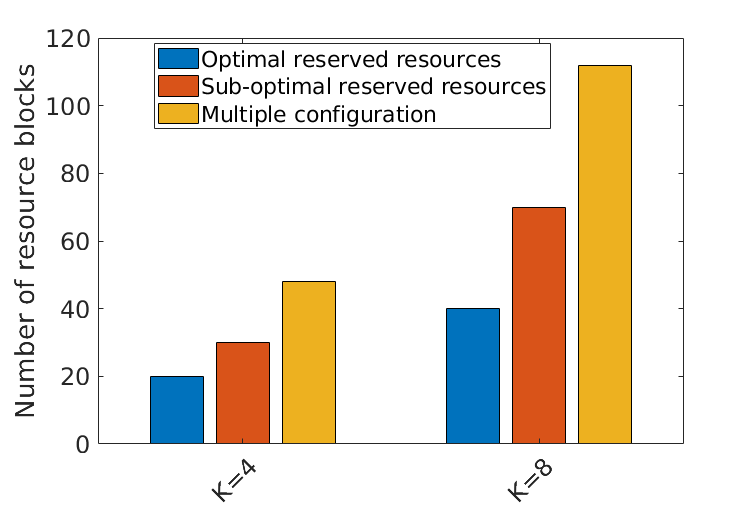
\includegraphics[scale=0.4]{fig19.png}}
\caption{Comparison of resource consumption.}
\label{fig19}
\vspace{-2mm}
\end{figure}

More comparisons of reserved resources' scheme with the conventional and other proposed schemes can be found in Table~\ref{tab8} and Table~\ref{tab9}.

\paragraph{SIC receiver is equipped at the gNB}\label{IVB2}

The parameters in the first scenario of \ref{IVB1} are used:  $M_1=10, K=4, N=28, P_{c1}=10^{-3}$. A SIC receiver is equipped at the gNB. 

Fig.~\ref{fig18} shows the error probability due to collision in the first reserved resource ($P_{col\_SIC\_1}$ in \eqref{eq15}) in terms of  the average number of random access events in an interval $\lambda$. When the gNB can decode more packets in the same block (L increases), the system can support much higher data rates while still achieving the same target reliability. In \ref{IVB1}, with $L=1$, the system only can support $\lambda=1.25\times10^{-4}$. But with $L=2$ or $L=3$, the system can support $\lambda=5.8\times10^{-3}$ or $\lambda=2.53\times10^{-2}$.

\begin{figure}[htbp]
\centerline{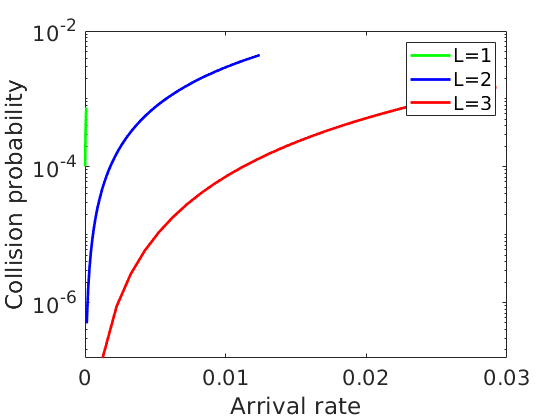
\includegraphics[scale=0.32]{fig18.png}}
\caption{The arrival rate vs collision probability.}
\vspace{-2mm}
\label{fig18}

\end{figure}

\subsubsection{Explicit feedback structure and additional SR in less-than-K-repetition transmission}

\begin{figure}[htbp]
\centerline{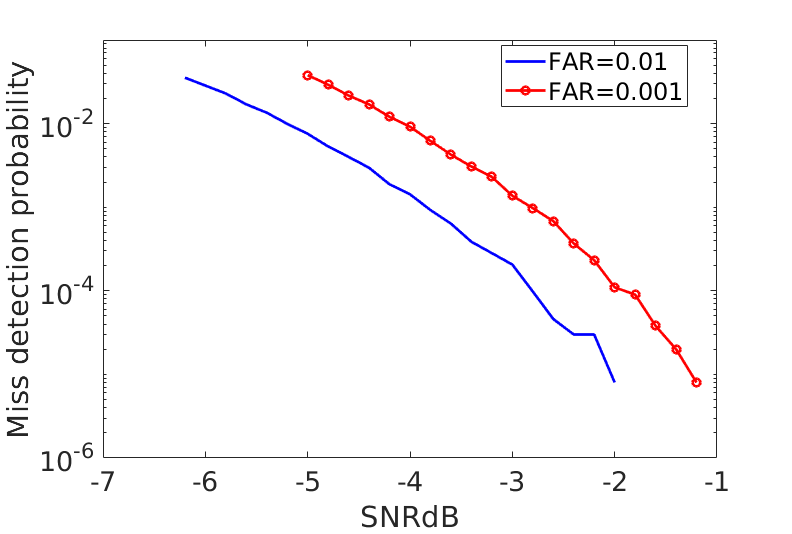
\includegraphics[scale=0.22]{fig15.png}}
\caption{DMRS detection performance.}
\vspace{-2mm}
\label{fig15}

\end{figure}

\begin{table*}[htbp]
\caption{Performance comparison of different schemes at $SNR = -5dB$ and $FAR = 0.001$}
\begin{center}
\begin{tabular}{|p{8em}|p{8em}|p{7em}|p{7em}|p{7em}|p{7em}|p{7em}|}
 \hline
 \textbf{Case}&\textbf{Scheme}&\textbf{Starting time offset (ms)}&\textbf{Number of repetitions}&\textbf{UE ID miss-detection probability}&\textbf{Number of retransmissions in UE ID miss-detection}&\textbf{Total UE ID miss-detection probability}\\
 \hline
 \multirow{5}{8em}{\centering {TB comes after the 1 \textsuperscript{st} CG occasion}} & Conventional transmission & $0$ & $3$ & $5.5\times10^{-5}$ & $0$ & $5.5\times10^{-5}$ \\\cline{2-7}
 & Conventional transmission with the UE waiting the next period & $0.75$ &$1$ &$0.038$ &$0$ & $0.038$ \\\cline{2-7}
 & Transmission with explicit feedback & $0$ &$3$ &$5.5\times10^{-5}$ &$0$ & $5.5\times10^{-5}$ \\\cline{2-7}
 & Transmission with SR& $0$ &$3$ &$2.1\times10^{-6}$ &$0$ & $2.1\times10^{-6}$ \\\cline{2-7}
   & Transmission with reserved resources& $0$ &$4$& $2.1\times10^{-6}$& $0$ & $2.1\times10^{-6}$ \\\cline{2-7}
\hline
  \multirow{5}{8em}{\centering {TB comes after the 2 \textsuperscript{nd} CG occasion}} & Conventional transmission & $0$ & $2$ & $10^{-3}$ & $0$ & $10^{-3}$ \\\cline{2-7}
 & Conventional transmission with the UE waiting the next period & $0.5$ &$2$ &$10^{-3}$ &$0$ & $10^{-3}$ \\\cline{2-7}
 & Transmission with explicit feedback & $0$ &$2$ &$10^{-3}$ &$1$ & $5.5\times10^{-5}$ \\\cline{2-7}
 & Transmission with SR& $0$ &$2$ &$5.5\times10^{-5}$ &$0$ & $5.5\times10^{-5}$ \\\cline{2-7}
   & Transmission with reserved resources& $0$ &$4$& $2.1\times10^{-6}$& $0$ & $2.1\times10^{-6}$ \\\cline{2-7}
 \hline
 \multirow{5}{8em}{\centering {TB comes after the 3 \textsuperscript{rd} CG occasion}} & Conventional transmission & $0$ & $1$ & $0.038$ & $0$ & $0.038$ \\\cline{2-7}
 & Conventional transmission with the UE waiting the next period & $0.25$ &$3$ &$5.5\times10^{-5}$ &$0$ & $5.5\times10^{-5}$ \\\cline{2-7}
 & Transmission with explicit feedback & $0$ &$1$ &$0.038$ &$2$ & $5.5\times10^{-5}$ \\\cline{2-7}
 & Transmission with SR& $0$ &$1$ &$10^{-3}$ &$0$ & $10^{-3}$ \\\cline{2-7}
   & Transmission with reserved resources& $0$ &$4$& $2.1\times10^{-6}$& $0$ & $2.1\times10^{-6}$ \\\cline{2-7}

%  increase row height, number of & = number of collumn
% &&&&&\\[-1em]
 
 \hline
\end{tabular}
\label{tab8}
\end{center}
\vspace{-6mm}
\end{table*}

The performance of DMRS detection is simulated with the parameters in Table~\ref{tab5}. Fig.~\ref{fig15} shows simulation results with different FAR. 

If the gNB cannot detect DMRS sequence, the packet is lost in the conventional feedback structure. It results in a degradation of UL transmission.

In the simulation system, HARQ process has periodicity $P$ equal to 4 slots. With SCS of 60 kHz, 4 slots spread in 1 ms. The configured number of repetition are 4. 3GPP Release 15 standardized that each slot has only one repetition \cite{ref3}. Thereby, 4 repetitions are carried out in 4 slots equal to one HARQ process. The sum of gNB processing time, feedback transmission time, UE processing time is one slot. The UE waits after one slot to decide whether dropping or retransmitting data.

Table~\ref{tab8} shows the performance of DMRS detection at SNR of -5dB and FAR of 0.001 in different schemes and arrival time of data. 

As can be seen, due to the constraint of HARQ process boundary, the UE might not transmit all 4 repetitions as configured if data comes late. Less repetitions transmitted means that DMRS miss-detection at the gNB increases. It leads to an increase of packet loss because the packet is assumed to be successful in timer-based feedback structure.

If the UE waits until the next HARQ process to transmit data, it might also not be able to do all the configured repetitions because of URLLC latency requirement.

Explicit feedback structure makes the UE retransmit data even if the gNB misses DMRS. It increases DMRS detection's performance and reduces packet loss. However, in one scenario as shown in Table~\ref{tab8}, after discovering that there is no ACK or UL grant, the UE cannot retransmit data because latency budget of 1 ms is reached.

An additional SR helps to reduce the probability of UE ID miss-detection. Nevertheless, if the actual number of repetitions are small as in in Table~\ref{tab8}, the miss-detection probability is still high compared to the case of full repetitions transmitted.

The utilization of reserved resources always guarantees the number of repetitions so the target reliability is ensured. However, resource consumption is higher than other schemes.

The advantages and disadvantages of three proposed schemes are summarized in Table~\ref{tab9}.

%\begin{table}[htbp]
%\caption{Performance comparison of different schemes when data comes after the first occasion in a period at $SNR = -5dB$ and $FAR = 0.001$}
%\begin{center}
%\begin{tabular}{|p{6em}|p{3em}|p{3em}|p{3.2em}|p{3.2em}|p{3.2em}|}
% \hline
% \textbf{Case} & \textbf{Starting time offset (ms)}&\textbf{Number of repetitions}&\textbf{UE ID miss-detection probability}&\textbf{Retrans in ID miss-detection}&\textbf{Total UE ID miss-detection probability}\\
% \hline
% Conventional transmission&$0$&$3$&$5.5\times10\textsuperscript{-5}$&$0$&$5.5\times10\textsuperscript{-5}$\\
% \hline
% Conventional transmission with the UE waiting the next period&$0.75$&$1$&$0.038$&$0$&$0.038$\\
% \hline
%Transmission with explicit ACK&$0$&$3$&$5.5\times10\textsuperscript{-5}$&$0$&$5.5\times10\textsuperscript{-5}$\\
%\hline
%Transmission with SR&$0$&$3$&$2.1\times10\textsuperscript{-6}$&$0$&$2.1\times10\textsuperscript{-6}$\\
% \hline
%Transmission with reserved resources&$0$&$4$&$2.1\times10\textsuperscript{-6}$&$0$&$2.1\times10\textsuperscript{-6}$\\
 %\hline
%\end{tabular}
%\label{tab6}
%\end{center}

%\end{table}

%\begin{table}[htbp]
%\caption{Performance comparison of different schemes when data comes after the second occasion in a period at $SNR = -5dB$ and $FAR = 0.001$}
%\begin{center}
%\begin{tabular}{|p{6em}|p{3em}|p{3em}|p{3.2em}|p{3.2em}|p{3.2em}|}
% \hline
% \textbf{Case} & \textbf{Starting time offset (ms)}&\textbf{Number of repetitions}&\textbf{UE ID miss-detection probability}&\textbf{Retrans in ID miss-detection}&\textbf{Total UE ID miss-detection probability}\\
% \hline
 %Conventional transmission&$0$&$2$&$10\textsuperscript{-3}$&$0$&$10\textsuperscript{-3}$\\
 %\hline
%Conventional transmission with the UE waiting the next period&$0.5$&$2$&$10\textsuperscript{-3}$&$0$&$10\textsuperscript{-3}$\\
% \hline
%Transmission with explicit ACK&$0$&$2$&$10\textsuperscript{-3}$&$1$&$5.5\times10\textsuperscript{-5}$\\
%\hline
%Transmission with SR&$0$&$2$&$5.5\times10\textsuperscript{-5}$&$0$&$5.5\times10\textsuperscript{-5}$\\
% \hline
% Transmission with reserved resources&$0$&$4$&$2.1\times10\textsuperscript{-6}$&$0$&$2.1\times10\textsuperscript{-6}$\\
%\hline
%\end{tabular}
%\label{tab7}
%\end{center}

%\end{table}

%\begin{table}[htbp]
%\caption{Performance comparison of different schemes when data comes after the third occasion in a period at $SNR = -5dB$ and $FAR = 0.001$}
%\begin{center}
%\begin{tabular}{|p{6em}|p{3em}|p{3em}|p{3.2em}|p{3.2em}|p{3.2em}|}
% \hline
 %\textbf{Case} & \textbf{Starting time offset (ms)}&\textbf{Number of repetitions}&\textbf{UE ID miss-detection probability}&\textbf{Retrans in ID miss-detection}&\textbf{Total UE ID miss-detection probability}\\
% \hline
% Conventional transmission&$0$&$1$&$0.038$&$0$&$0.038$\\
 %\hline
%  Conventional transmission with the UE waiting the next period&$0.25$&$3$&$5.5\times10\textsuperscript{-5}$&$0$&$5.5\times10\textsuperscript{-5}$\\
% \hline
%Transmission with explicit ACK&$0$&$1$&$0.038$&$2$&$5.5\times10\textsuperscript{-5}$\\
%\hline
%Transmission with SR&$0$&$1$&$10\textsuperscript{-3}$&$0$&$10\textsuperscript{-3}$\\
% \hline
% Transmission with reserved resources&$0$&$4$&$2.1\times10\textsuperscript{-6}$&$0$&$2.1\times10\textsuperscript{-6}$\\
% \hline
%\end{tabular}
%\label{tab8}
%\end{center}

%\end{table}


\begin{table}[htbp]
\caption{Comparison of three proposed schemes}
\begin{center}
\begin{tabular}{|p{4em}|p{11em}|p{11em}|}
 \hline
& \textbf{Advantage}&\textbf{Disadvantage}\\
 \hline
 Reserved resources &+ Ensure the configured number of repetitions & + Resource consumption of reserved resource\\ & + Optimal sizes of reserved resources &+ Overhead of signal to configure reserved resources\\
 \hline
  Explicit feedback structure& + Avoid packet loss due to DMRS miss-detection&+ Resource consumption of ACK feedback\\& &+ Latency constraint limits the number of retransmissions\\
 \hline
Additional SR&+ Enhance UE ID detection&+ Resource consumption of SR\\& &  + High UE ID miss-detection if the number of packets transmitted are small\\

%  increase row height, number of & = number of collumn
% &&&&&\\[-1em]
 
 \hline
\end{tabular}
\label{tab9}
\end{center}
\vspace{-6mm}
\end{table}






\section{Conclusion}

URLLC requires strict reliability and latency requirements but there are still problems in physical layer design that make the system unable to achieve those requirements. The techniques proposed in this paper helps the URLLC transmissions overcome two major problems: first is the successfull eMBB and URLLC multiplexing, the second is to ensure QoS targets when URLLC UEs can not transmit less than K repetitions with CG transmissions. 

In the problem of multiplexing between eMBB and URLLC UEs, a mechanism using PI avoids the collision between the GB eMBB and URLLC UEs. This mechanism chooses the eMBB candidates for cancellation and informs these UEs by 1-bit flag embedded in UL grant. The UEs that receive an active flag increase monitoring periodicity and capability. Besides that, an overlap indication with explicit feedback or additional SR are used to enhance the performance of CG URLLC multiplexing with GB eMBB. The simulation shows that these techniques reduce URLLC packet loss due to DMRS miss-detection in the transmission suffering from the interference from the eMBB UEs. 

For the problem of less than the configured number of repetitions, three techniques, the optimal reserved resources, explicit feedback and additional SR, are proposed over the prior art. The advantages and disadvantages of each method have been shown by the calculation and simulations.  

\section*{Acknowledgment}

This work was supported in part by TCL and H2020 project 5GENESIS (5genesis.eu).

\begin{thebibliography}{00}

\bibitem{ref1} 3GPP TR 38.913 v15.0.0, ``Study on scenarios and requirements for next generation access technologies.''
\bibitem{ref2} Huawei, HiSilicon, Nokia, Nokia Shanghai Bell, ``New SID on Physical Layer Enhancements for NR URLLC''. 3GPP RP-182089, TSG-RAN\#81, Gold Coast, Australia, Sept 10--13, 2018.
\bibitem{ref3} 3GPP TS 38.211 v15.3.0, ``Physical channels and modulation.''
\bibitem{ref4} 3GPP TR 38.802 v14.2.0, ``Study on new radio access technology physical layer aspects.''
\bibitem{ref5} 3GPP TS 38.214 v15.3.0, ``Physical layer procedures for data.''
\bibitem{ref20} Draft report of 3GPP TSG RAN WG1 \#97, Reno, USA, May 13--17, 2019
\bibitem{ref6} 3GPP TS 38.331 v15.3.0, ``Radio Resource Control (RRC) protocol specification.''
\bibitem{ref7} Draft report of 3GPP TSG RAN WG1 \#95, Spokane, USA, Nov 12--16, 2018
\bibitem{ref8} Ericsson, ``Enhancement of Configured Grant for NR URLLC'', 3GPP R1-1812162, RAN1\#95, Spokane, USA, November 12--16, 2018.
\bibitem{ref9} Huawei, HiSilicon, ``Enhanced UL configured grant transmissions'', 3GPP R1-1812226, RAN1\#95, Spokane, USA, November 12--16, 2018.
\bibitem{ref10} R. breu, G. Berardinelli, T. Jacobsen, K. Pedersen and P. Mogensen, ``A Blind Retransmission Scheme for Ultra-Reliable and Low Latency Communications'', 2018 IEEE 87th Vehicular Technology Conference (VTC Spring), June 2018.
\bibitem{ref11} Z. Zhou, R. Ratasuk, N. Mangalvedhe and A. Ghosh, ``Resource Allocation for Uplink Grant-Free Ultra-Reliable and Low Latency Communications'', 2018 IEEE 87th Vehicular Technology Conference (VTC Spring), June 2018.
\bibitem{ref12} B. Singh, O. Tirkkonen, Z. Li and M. A. Uusitalo, ``Contention-Based Access for Ultra-Reliable Low Latency Uplink Transmissions'',  IEEE Wireless Communications Letters, April 2018.
\bibitem{ref13} Huawei, HiSilicon, ``UL inter-UE transmission prioritization and multiplexing'', 3GPP R1-1810158, RAN1\#94bis, Spokane, Chengdu, China, 8--12 October, 2018.
\bibitem{ref14} ZTE, ``UL inter-UE multiplexing between eMBB and URLLC'', 3GPP R1-1900074, RAN1 AH 1901, Taipei,  21--25 January, 2019.
\bibitem{ref15}  Sony, ``Inter-UE uplink multiplexing of URLLC \& eMBB traffics'', 3GPP R1-1812745, RAN1\#95, Spokane, USA, November 12--16, 2018.
\bibitem{ref16}  Institute for Information Industry (III), ``UL Inter UE Tx prioritization/multiplexing'', 3GPP R1-1813481, RAN1\#95, Spokane, USA, November 12--16, 2018.
\bibitem{ref17}  NEC, ``UL inter-UE multiplexing of eMBB and URLLC'', 3GPP R1-1812419, RAN1\#95, Spokane, USA, November 12--16, 2018.
\bibitem{ref18}  C.-P. Li, J. Jiang, W. Chen, T. Ji, and J. Smee, ``5G ultra-reliable and low-latency systems design,'' in 2017 European Conference on Networks and Communications (EuCNC), Jun. 2017, pp. 1-5. 
\bibitem{ref19} D. Tse and P. Viswanath, Fundamentals of Wireless Communication. Cambridge University Press, 2005. 
\bibitem{ref21} C. Stefanovic, E. Paolini, and G. Liva, ``Asymptotic performance of coded slotted aloha with multipacket reception,'' IEEE Communications Letters, vol. 22, no. 1, pp. 105--108, 2018.
\bibitem{b9} Trung-Kien Le, Umer Salim, Florian Kaltenberger, ``Optimal reserved resources to ensure the repetitions in Ultra-Reliable Low-Latency Communication Uplink Grant-free transmission'',  2019 European Conference on Networks and Communications (EuCNC), June 2019.
\bibitem{ad100} Trung-Kien Le, Umer Salim, Florian Kaltenberger, ``Strategies to meet the configured repetitions in URLLC Uplink Grant-Free transmission'',  2019 16th International Symposium on Wireless Communication Systems (ISWCS), August 2019.
\bibitem{ad99} Trung-Kien Le, Umer Salim, Florian Kaltenberger, ``Improving Ultra-Reliable Low-Latency Communication in multiplexing with Enhanced Mobile Broadband in grant-free resources'', 2019 IEEE International Symposium on Personal, Indoor and Mobile Radio Communications (PIMRC), September 2019.
\bibitem{ad101} Trung-Kien Le, Umer Salim, Florian Kaltenberger, ``Control and data channel combining in Ultra-Reliable Low-Latency Communication'', Asilomar Conference on Signals, Systems, and Computers, November 2019.
\end{thebibliography}


\begin{IEEEbiography}[{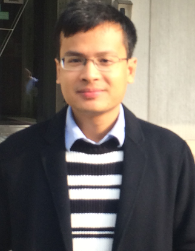
\includegraphics[width=1in,height=1.25in,clip,keepaspectratio]{a1.PNG}}]{Trung-Kien Le} received MCS. degree specializing in Mobile Computing Systems from EURECOM, France. Currently, he is a PHD student in Sorbonne University and  EURECOM. His research interest is Ultra Reliable Low Latency Communication in 5G New Radio.
\end{IEEEbiography}

\begin{IEEEbiography}[{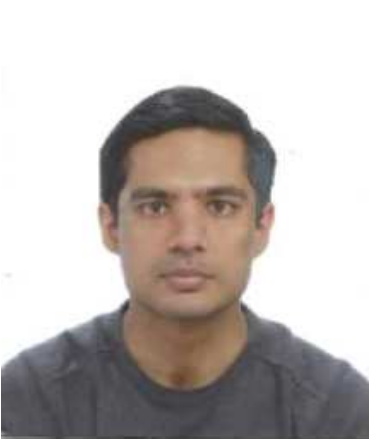
\includegraphics[width=1in,height=1.25in,clip,keepaspectratio]{a2.png}}]{Umer Salim} received his Ph.D. and M.S. degrees, specializing in communication theory and signal processing from Eurecom and Supelec, France, respectively. He is currently working at TCL Communications as 5G Systems Architect and 3GPP RAN1 delegate for 5G standardization activity. Before joining TCL, he worked at Intel Mobile Communications designing modems for high end smart phones and tablets. He has several years of research experience in physical layer of wireless communications.
\end{IEEEbiography}

\begin{IEEEbiography}[{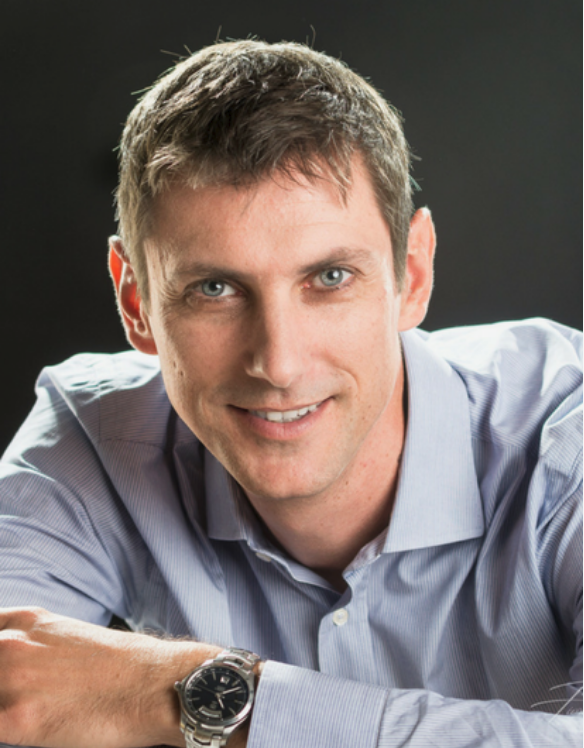
\includegraphics[width=1in,height=1.25in,clip,keepaspectratio]{a3.png}}]{Florian Kaltenberger} (S05-M08) received his Dipl.-Ing. degree and his Ph.D. degree both in technical mathematics from the Vienna University of Technology in 2002 and 2007, respectively. He is an assistant professor at the Communication Systems Department of Eurecom, Sophia-Antipolis, France, and part of the management team of the real time open-source 5G platform OpenAirInterface.org. From 2003 to 2007 he was with the Wireless Communications Group of the Austrian Research Centers, where he was developing a real-time MIMO channel emulator. His research interests include 5G and MIMO systems at large, software defined radio, signal processing for wireless communications, as well as channel modeling and simulation.
\end{IEEEbiography}

\EOD

\end{document}
